% !TEX root = main.tex
\label{ch:data_hpc}
In \S~\ref{sec:pilot-data-hadoop}, we explore the integration between Hadoop and HPC resources utilizing the Pilot-Abstraction allowing application to manage HPC (e.\,g.\ simulations) and data-intensive application stages in a uniform way.
We propose two extensions to RADICAL-Pilot: the ability to spawn and manage Hadoop/Spark clusters on HPC infrastructures on demand (Mode I), and to connect and utilize Hadoop and Spark clusters for HPC applications (Mode II).
Both extensions facilitate the complex application and resource management requirements of data-intensive applications that are best met by a best-of-bread mix of Hadoop and HPC. 
By supporting these two usage modes, RADICAL-Pilot dramatically simplifies the barrier of deploying and executing HPC and Hadoop/Spark side-by-side.

In \S~\ref{sec:task-par}, we investigate three task-parallel frameworks and their suitability for implementing MD trajectory analysis algorithms.
In addition to Spark and Dask, we investigate RADICAL-Pilot~\cite{merzky2019using}, a Pilot-Job~\cite{luckow2012pstar} framework designed for implementing task-parallel applications on HPC.
We utilize MPI4py~\cite{dalcin2005mpi} to provide MPI equivalent implementations of the algorithms.
The task-parallel implementations performance and scalability compared to MPI is the basis of our analysis.
MD trajectories are time series of atoms/particles positions and velocities, which are analyzed using different statistical methods to infer certain properties, e.\,g. the relationship between distinct trajectories, snapshots of a trajectory etc.
As a result, they can be considered as a representative set of scientific datasets that are organized as time series and their analysis algorithms. 

The paper makes the following contributions: 
\begin{inparaenum}[i)]
    \item it characterizes and explains the behavior of different MDAnalysis algorithms on these frameworks, and
    \item provides a conceptual basis for comparing the abstraction, capabilities and performance of these frameworks.
\end{inparaenum}


\section{Integrating Hadoop and Spark with HPC workload management system}
% !TEX root = main.tex
\label{ch:pilot-data-hadoop}

Computational campaigns on High Performance Computing (HPC) resources can execute compute- or data- intensive workflows and applications.
Compute-intensive applications and workflows are associated with either a single long running executable or an ensemble of compute-intensive tasks~\cite{balasubramanian2018harnessing}.
On the other hand, data-intensive applications are associated with multiple stages of execution which can I/O, memory and compute bound.
While MPI is the most common programming model for compute-intensive applications, the MapReduce~\cite{dean2004mapreduce} abstraction is commonly used for data-intensive applications~\cite{hellerstein2012science}.

%However, HPC resources are designed to support mainly compute-intensive long-running MPI applications, as they offer
%Not surprisingly, HPC resource architectures offer large number of computing resources, e.g., CPUs and GPUs, connected by high-end networks (e.\,g.\ Infiniband) and filesystems, such as Lustre and PVFS.
%They have however limitations in supporting data-intensive and I/O bound workflows.

Hadoop~\cite{hadoop} popularized the use of MapReduce~\cite{dean2004mapreduce} for data-intensive applications.
Hadoop's distirbuted filesystem (HDFS) automatically partitions data and distributes them to different nodes in a distributed cluster.
In addition, Hadoop's engine takes advantage of data-locality and transfers computations to nodes allowing to process data in parallel while reducing data transfers.
While Hadoop simplified the processing of vast volumes of data, it has limitations in its expressiveness~\cite{yelick2011magellan,isard2007dryad}.
The complexity of creating sophisticated applications such as iterative machine learning algorithms required multiple MapReduce jobs and persistence to Hadoop's Filesystem (HDFS) after each iteration.
This lead to several higher-level abstractions for implementing sophisticated data pipelines.

The most well-known processing framework in the Hadoop ecosystem is Spark~\cite{zaharia2010spark}.
In contrast to MapReduce, it provides a richer API, more language bindings and a memory-centric processing engine that can utilize distributed memory and retain resources across multiple task generations.
Spark's \emph{Reliable Distributed Dataset (RDD)} ~\cite{zaharia2012resilient} abstraction provides a powerful way to manipulate distributed collections stored in cluster nodes' memory.
Spark is used for building complex data workflows and advanced analytic tools, such as MLLib~\cite{mllib}.
Although the addition/development of new and higher-level execution frameworks addressed some of the problems of data processing, it introduced the problem of heterogeneity of access and resource management.

% Problem statement.
Some computational campaigns cannot be easily classified as only compute- or data-intensive, such as bio-molecular dynamics~\cite{dror2012biomolecular}.
Bio-molecular simulations are now high-performant, reach increasing time scales and problem sizes, and thus generating immense amounts of data.
Often times the data generated needs to be analyzed so as to determine the next set of simulation configurations.
Several tools evolved to meet the demand for molecular dynamics data analysis, such MDAnalysis~\cite{michaud2011mdanalysis,gowers2016mdanalysis}, CPPTraj~\cite{roe2013ptraj} and HiMach~\cite{tiankai2008scalable}.
Although these tools offer domain-specific analytics, scaling them to high data volumes remains a challenge.
This points to the need for environments that support scalable data processing while preserving the ability to run simulations at the scale so as to generate the data.
To the best of our knowledge, there does not exist a solution that provides the integrated capabilities of Hadoop and HPC.

% Solution
In this chapter, we explore the integration between Hadoop~\cite{hadoop}, and Spark~\cite{zaharia2010spark} and HPC resources.
We utilize the Pilot-Abstraction~\cite{luckow2012pstar} allowing to manage HPC and data-intensive applications in a uniform way.
We explore two extensions to RADICAL-Pilot~\cite{merzky2018design}, a Pilot-Job~\cite{luckow2012pstar} runtime system designed for implementing task-parallel applications on HPC: 
\begin{inparaenum}[1)]
    \item the ability to spawn and manage Hadoop/Spark clusters on HPC infrastructures on demand (Mode I); and
    \item to connect and utilize Hadoop and Spark clusters for HPC applications (Mode II)
\end{inparaenum}.
Both extensions facilitate the complex application and resource management requirements of data-intensive applications.
By supporting these two usage modes, RADICAL-Pilot dramatically simplifies the barrier of deploying and executing HPC and Hadoop/Spark workflows side-by-side.

The chapter is organized as follows: In section~\ref{sec:hpc_hadoop_rel} we discuss the current solutions and challenges of integrating data analytics and HPC.
We continue with discussing the modes of integration and interoperability between data analytics and HPC in \S~\ref{sec:integration_mode} and the experimental validations of the integration in ~\S~\ref{sec:rph-exps}.
The chapter closes with our conclusions in section~\ref{sec:hpc_hadoop_concl}.

\section{Related Work and Challenges}
\label{sec:hpc_hadoop_rel}
\subsection{Related Work}
There are several frameworks which explored the usage of Hadoop on HPC resources, e.\,g., Hadoop on Demand~\cite{hod}, JUMMP~\cite{moody2013jummp}, MagPie~\cite{chu2015magpie}, MyHadoop~\cite{krishnan2011myhadoop}, MyCray~\cite{mycray}.
These frameworks provide users with a set of scripts that can spawn and manage a Hadoop cluster on HPC resources.
As soon as Hadoop is started, users can either submit their MapReduce jobs interactively or via a script.

Although these frameworks can spawn and manage Hadoop clusters, they isolate the Hadoop cluster from the HPC environment.
The scripts and capabilities they offer interact directly with the HPC's submission system.
As a result, users cannot execute on the same set of nodes HPC and Hadoop applications.
Further, they do not necessarily optimize configurations and resource usage, including the use of available SSDs, parallel filesystems and high-end network features, e.\,g.\ RDMA~\cite{rahman2014homr}.

\subsection{Challenges}
Hadoop originally provided a rudimentary resource management system, the YARN scheduler.
The YARN scheduler~\cite{vavilapalli2013apache} provides an application-level scheduling framework addressing the increased requirements with respect to applications and infrastructure, such as more complex data localities (memory, disk, datacenter), long-lived services, periodic jobs, interactive and batch jobs.
In contrast, to batch schedulers of HPC resources, YARN is optimized for supporting data-intensive environments and managing a large number of fine-grained tasks.

While YARN manages system-level resources, applications need to implement an application-level scheduler that optimizes their specific requirements, e.,g., with respect to data locality.
This application-level scheduler, the \textit{Application Master}, is responsible for allocating resources ---called containers---  and executing tasks on these resources.
In addition, the Application Master manages data locality, e.,g., between HDFS blocks and container locations, by allocating containers on specific nodes.

Managing resources on top of YARN is associated with several challenges.
While applications with fine-grained, short-running tasks are well supported, applications with coarse-grained, long-running task, such as MPI applications, are not.
To achieve interoperability and integration between Hadoop and HPC, it is essential to consider a more diverse set of applications on top of YARN.

A particular challenge for Hadoop on HPC deployment is the choice of storage and filesystem backend.
Typically, when using Hadoop local storage is preferred.
Nevertheless, in some cases, e.\,g.\ processing many small files, random data access is required or the number of parallel tasks is low to medium, using a parallel filesystem can yield a better performance.
For this purpose, many parallel filesystems provide a special client library which improves the interoperability with Hadoop, but limits data locality and any data placement optimization.

Another challenge is the integration between both HPC and Hadoop environments.
Rather than preserving HPC and Hadoop ``environments'' as software silos, there is a need for an approach that integrates them. 
We utilize the Pilot-Abstraction as a unifying concept to efficiently support the integration, and not just the interoperability between HPC and Hadoop.
By utilizing the multi-level scheduling capabilities of YARN, the Pilot-Abstraction can efficiently manage Hadoop resources providing an application with the means to reason about data, compute resources and allocation.
In addition, we show how the Pilot-Abstraction can be used to manage Hadoop applications on HPC environments.

The Pilot-Abstraction~\cite{luckow2012pstar} is successfully used on HPC resources supporting a diverse set of task-based workflows.
A Pilot-job is a placeholder job which is submitted to the resource management system and represents a container for a dynamic set of tasks.
Pilot-jobs are, also, a well-known example of multi-level scheduling, which is often used to separate system-level resource and user-level workload management.
The Pilot-Abstraction defines the following entities:
\begin{inparaenum} [1)]
    \item a Pilot which allocates a set of computational resources (e.\,g.\,cores); and
    \item  a Compute-Unit (CU) as a self-contained piece of work represented as an executable.
\end{inparaenum}
The Pilot-Abstraction has been implemented within RADICAL-Pilot~\cite{merzky2018design}.


\section{Data analytics and HPC integration: RADICAL-Pilot and YARN/ Spark}
\label{sec:integration_mode}
Having established the potential of the Pilot~-Abstraction for a range of high-performance applications~\cite{treikalis2016repex,ragothaman2014developing,ko2014numerical}, we use it as the starting point for integrating HPC and data-intensive analytics.
As depicted in Figure~\ref{fig:figures_hadoop-on-hpc-viceverse}, there are at least two different usage modes to consider:
\begin{inparaenum}[1)]
    \item Mode I: Running Hadoop/Spark applications on HPC environments (Hadoop on HPC),
    \item Mode II: Running HPC applications on YARN clusters (HPC on Hadoop).
\end{inparaenum}

\begin{figure}[t]
    \centering
    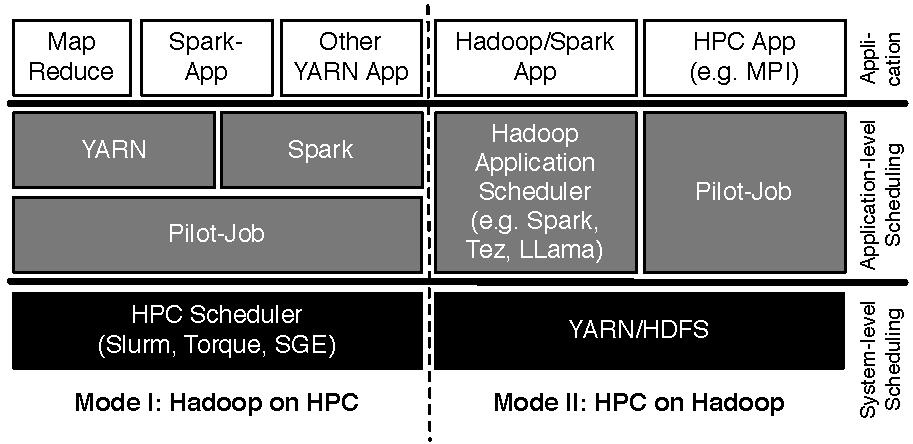
\includegraphics[width=.85\textwidth]{figures/data_analytics_hpc/hpc_hadoop/hadoop-on-hpc-viceverse.pdf}
    \caption{Hadoop and HPC Interoperability modes\label{fig:figures_hadoop-on-hpc-viceverse}}
\end{figure}

Mode I is critical to support traditional HPC environments so as to support applications with both compute and data requirements.
Mode II is important for cloud environments (e.\,g.\ Amazon's Elastic MapReduce) and an emerging class of HPC machines with new architectures and usage modes, such as Wrangler~\cite{wrangler}, that support Hadoop natively.
For example, Wrangler supported dedicated Hadoop environments (based on Cloudera Hadoop 5.3) via a reservation mechanism.
%We discuss, the integration of Hadoop and Spark runtimes into RADICAL-Pilot, which enables both the interoperable use of HPC and Hadoop, as well as the integration of HPC and Hadoop applications (Mode I and II).
Using these new capabilities, applications can seamlessly connect HPC stages (e.\,g.\ simulation stages) with analysis staging using the Pilot-Abstraction to provide unified resource management.
%\subsection{Mode I---II: }
%\label{ssec:rp-impl}

With the introduction of YARN, a broader set of applications can be executed within a Hadoop cluster than earlier.
However, developing and deploying YARN applications potentially side-by-side with HPC applications remains a difficult task.
Established abstractions which are easy to use while enabling users to reason about compute and data resources across infrastructure types (i.\,e.\ Hadoop, HPC and clouds) are missing. 

Schedulers such as YARN effectively facilitate application-level scheduling.
Although, the development efforts for YARN applications are still high.
YARN provides a low-level abstraction for resource management, e.g., a Java API and protocol buffer specification.
Typically interactions between YARN and applications are much more complex than the interactions between an application and an HPC scheduler.
Further, applications must be able to run on a dynamic set of resources; YARN e.\,g.\ can preempt containers in high-load situations.
Data/compute locality need to be manually managed by the application scheduler by requesting resources at the location of a file chunk.
Also, the scheduler can preempt resources (the so called YARN containers).

To address these shortcomings, various frameworks that aid the development of YARN applications have been proposed.
Llama~\cite{llama} offers a long-running application master for YARN designed for the Impala SQL engine.
Apache Slider~\cite{apache-slider} supports long-running distributed application on YARN with dynamic resource needs allowing applications to scale to additional containers on demand.
While these frameworks simplify development, they do not address concerns such as interoperability and integration of HPC/Hadoop.
Integrating YARN and RADICAL-Pilot (RP) allows applications to run HPC and YARN applications on HPC resources concurrently.

\subsubsection*{RADICAL-Pilot and YARN Overview}
\label{sssec:rp_yarn}
% RADICAL-Pilot Overview
Figure~\ref{fig:comp_rp_arch} illustrates the architecture of RADICAL-Pilot and the components that were extended.
The figure on the left shows the macro architecture of RADICAL-Pilot.
The figure on the right shows the architecture of the Pilot-Agent which is a critical functional component.
RADICAL-Pilot consists of a client module with the Pilot-Manager and Unit-Manager and a set of RADICAL-Pilot-Agents running on resources.
The Pilot-Manager is the central entity responsible for managing a set of pilots.
Pilots are described via a Pilot description, which contains the pilot's resource requirements and is submitted to the Pilot-Manager.
The Pilot-Manager, then, submits a placeholder job which will run the RADICAL-Pilot-Agent via the Resource Management System using the SAGA-API~\cite{merzky2015saga} (steps P.1-P.2).
Subsequently, the Unit-Manager and the RADICAL-Pilot-Agent manage the application workload (the Compute-Units,steps U.1-U.7)~\cite{merzky2019using}.

\begin{figure}
    \centering
    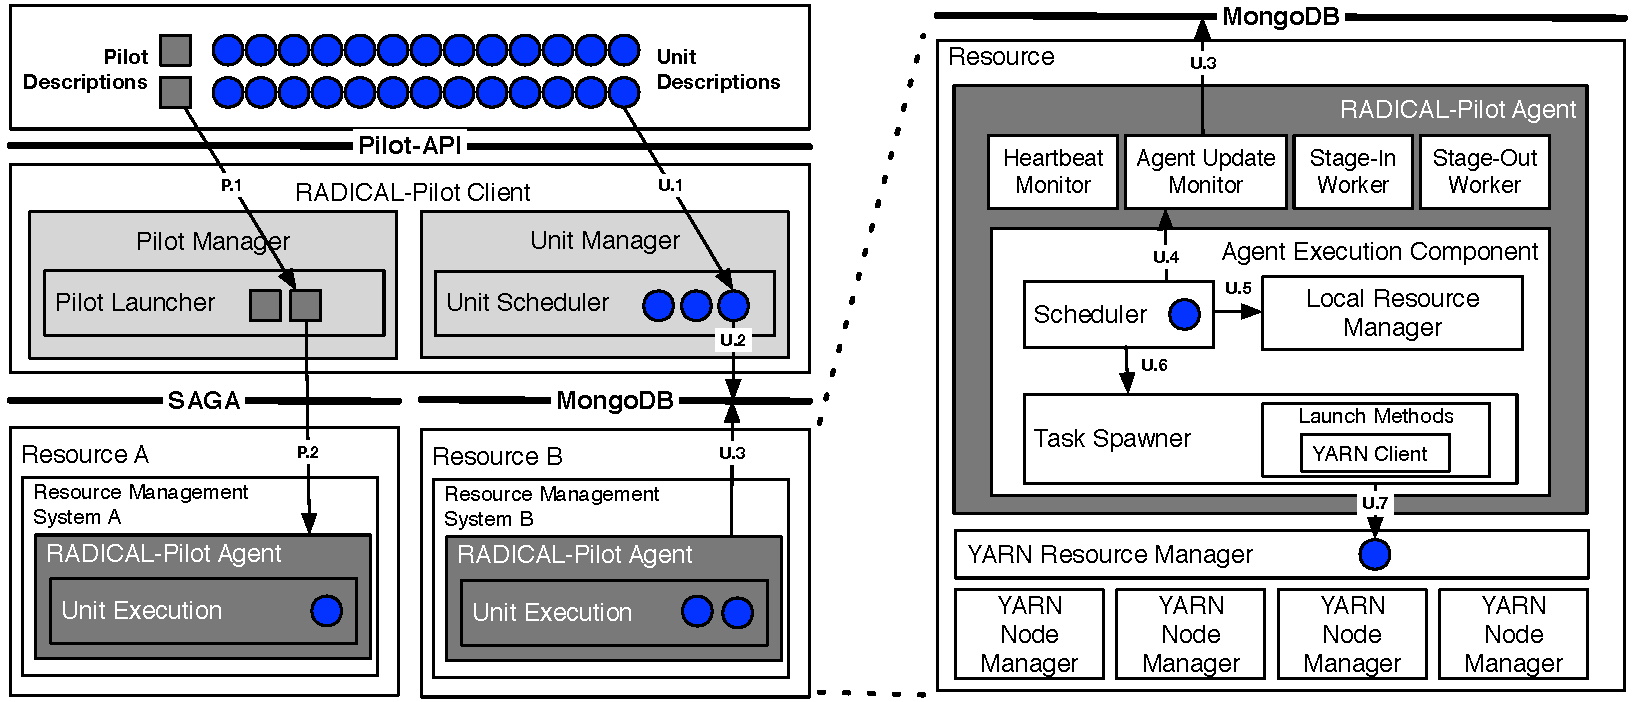
\includegraphics[width=0.85\textwidth]{figures/data_analytics_hpc/hpc_hadoop/rp-architecture-yarn.pdf}
    \caption{\textbf{RADICAL-Pilot and YARN Integration:} There are two main interactions between the application and RADICAL-Pilot -- the management of Pilots (P.1-P.2) and the management of Compute Units (U.1-U.7).  All YARN specifics are encapsulated in the RADICAL-Pilot-Agent.\label{fig:comp_rp_arch}}
\end{figure}

The RADICAL-Pilot-Agent has a modular and extensible architecture and consists of the following components: the Agent Execution Component, Heartbeat Monitor, Agent Update Monitor, Stage In and Stage Out Workers.
The main integration of YARN and RP is done in the Agent Execution Component.
This component consist of four sub-components:
\begin{inparaenum}[a)]
    \item the \textit{scheduler} is responsible for monitoring the resource usage and assigning CPUs/GPUs to Compute Units;
    \item the \textit{Local Resource Manager} (LRM) interacts with the batch system and communicates to the pilot the available number of computing resources and how they are distributed;
    \item the \textit{Task Spawner/ Executor} configures the execution environment, executes and monitors each unit; and
    \item the \textit{Launch Method} encapsulates the environment specifics for executing an application, e.\,g.\ the usage of \texttt{mpiexec} for MPI applications, machine-specific launch methods (e.g. \texttt{aprun} on Cray machines) or the usage of YARN.
\end{inparaenum}
After unit completes its execution, the Task Spawner collects the exit code, standard output, and informs the scheduler about the freed cores.

\subsubsection*{RADICAL-Pilot and YARN Integration}
\label{sssec:rp-yarn}

There are two integration options for RADICAL-Pilot and YARN: (i) Integration on Pilot-Manager level, via a SAGA adaptor, and (ii) integration on the RADICAL-Pilot-Agent level.
The first approach is associated with several challenges: firewalls typically prevent the communication between external machines and a YARN cluster.
A YARN application is not only required to communicate with the resource manager, but also with the node managers and containers.
Further, this approach would require significant extension of the Pilot-Manager, which currently relies on the SAGA Job API for launching and managing pilots.
Capabilities like on-demand provisioning of a YARN cluster and complex application-resource management protocol required by YARN are difficult to abstract behind the SAGA API.

The second approach encapsulates YARN specifics on resource-level and a YARN cluster is decentrally provisioned.
Units are scheduled and submitted to the YARN cluster via the Unit-Manager and the RADICAL-Pilot-Agent scheduler.
By integrating at the RADICAL-Pilot-Agent level, RADICAL-Pilot supports both Mode I and II as outlined in Figure~\ref{fig:figures_hadoop-on-hpc-viceverse}.

As illustrated in Figure~\ref{fig:comp_rp_arch}, RADICAL-Pilot  (steps P.1 and P.2) starts on the remote resource using SAGA.
In Mode I, during the launch of the RADICAL-Pilot-Agent a YARN cluster is spawned on the allocated resources (Hadoop on HPC), while in Mode II the RADICAL-Pilot-Agent connects to a YARN cluster running on the resources of the RADICAL-Pilot-Agent.
Once the RADICAL-Pilot-Agent is started, it accepts Compute Units submitted via the Unit-Manager (step U.1).
The Unit-Manager queues new Compute Units using a shared MongoDB (step U.2).
The RADICAL-Pilot-Agent periodically checks for new Compute Units (U.3) and queues them in the scheduler (U.4).
Finally, the Executor manages the execution of the Compute Units (step U.6 and U.7).

The \emph{Local Resource Manager (LRM)} provides an abstraction to local resource details for other components of the RADICAL-Pilot-Agent.
The LRM evaluates the environment variables provided by the resource management systems to obtain information, such as the number of cores per node, memory and the assigned nodes.
This information can be accessed through the Resource Manager's API.
In Mode I (Hadoop on HPC), during the initialization of the RADICAL-Pilot-Agent, the LRM setups the HDFS and YARN daemons.
First, the LRM downloads Hadoop and creates the necessary configuration files, i.\,e. the \texttt{mapred-site.xml}, \texttt{core-site.xml}, \texttt{hdfs-site.xml}, \texttt{yarn-site.xml} and the slaves and master file containing the allocated nodes.
The node that is running the Agent, runs the master daemons of Hadoop: the HDFS Namenode and the YARN Resource Manager.
After the configuration files are written, HDFS and YARN are started and meta-data about the cluster, i.\,e.\ the number of cores and memory, are provided to the scheduler.
They remain active until all the tasks are executed.
Before termination of the agent, the LRM stops the Hadoop and YARN daemons and removes the associated data files.
In Mode II (Hadoop on HPC), the LRM solely collects the Hadoop cluster resource information.

The \emph{scheduler} is another extensible component of the RADICAL-Pilot-Agent responsible for queuing compute units and assigning them to resources.
To support YARN, we created a special scheduler that utilizes the cluster state information (e.\,g.\ the amount of available cores, memory, queue information, application quotas etc.) obtained via the YARN's Resource Manager's REST API.
In contrast to other RADICAL-Pilot schedulers, it specifically utilizes memory in addition to cores for assigning resources to Compute Units.

The \emph{Task Spawner} is responsible for managing and monitoring the execution of a Compute Unit.
The \emph{Launch Method} component encapsulates resource/launch-method specific operations, e.\,g.\ the usage of the \texttt{yarn} command line tool for submitting and monitoring applications.
After the launch of a Compute Unit, the Task Spawner periodically monitors its execution and updates its state in the shared MongoDB instance by utilizing the application log file.

\begin{figure}[t]
    \centering
    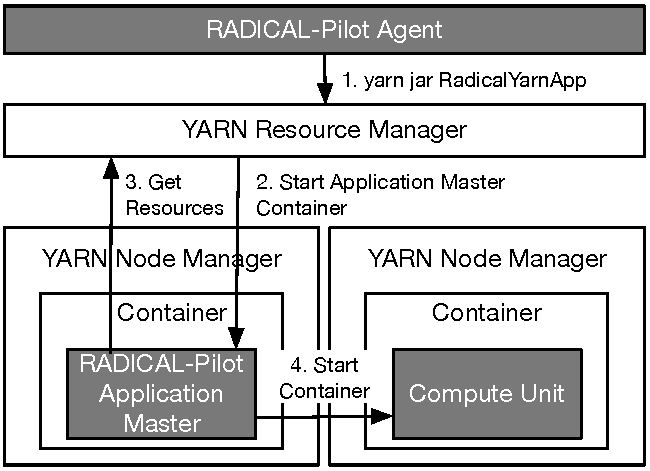
\includegraphics[width=.65\textwidth]{figures/data_analytics_hpc/hpc_hadoop/yarn.pdf}
    \caption{RADICAL-Pilot YARN Agent Application.}
%    \caption{\textbf{RADICAL-Pilot YARN Agent Application: }
%        RADICAL-Pilot provides a YARN application that manages the execution of Compute Units.
%        The application is initialized with parameters defined in the Compute Unit Description and started by the Task Spawner (step 1/2).
%        The Application Master requests resources from the Resource Manager and starts a container running the Compute Unit (step 3/4).}
    \label{fig:figures_yarn}
\end{figure}

\emph{RADICAL-Pilot Application Master:}
A particular integration challenge is the multi-step resource allocation process imposed by YARN depicted in Figure~\ref{fig:figures_yarn}, which differs significantly from HPC schedulers.
The central component of a YARN application is the Application Master, which is responsible for negotiating resources with the YARN Resource Manager as well as managing the execution of an application in the assigned resources.
The unit of allocation in YARN is a container~\cite{murthy2014apache}.
The YARN client (part of the YARN Launch Method) implements a YARN Application Master, which is the central instance for managing the resource requirements of an application.
RADICAL-Pilot utilizes a managed application master that is run inside a YARN container.
Once the Application Master container is started, it is responsible for requesting a YARN container meeting the resource requirements of the Compute Unit from the YARN's Resource Manager.
Once YARN allocates a set of containers, the CU starts inside these containers.
A wrapper script responsible for setting up a RADICAL-Pilot environment, staging of the specified files and running the executable defined in the Compute Unit Description, is used for this purpose.
Every Compute Unit is mapped to a YARN application consisting of an Application Master and a container of the size specified in the Compute Unit Description.

\subsubsection*{RADICAL-Pilot and Spark Integration}
\label{sssec:rp_spark}
Spark offers multiple deployment modes: standalone, YARN and Mesos.
While it is possible to support Spark on top of YARN, this approach is associated with significant complexity and overhead as two instead of one framework need to be configured and bootstrapped.
Since RADICAL-Pilot operates in user-space and single-user mode, no advantages with respect to using a multi-tenant YARN cluster environment exist.
Thus, we support Spark via the standalone deployment mode.

Similar to the YARN integration, the necessary changes for Spark are confined to the RADICAL-Pilot-Agent.
Similarly, the Local Resource Manager is responsible for initialization and deployment of the Apache Spark environment.
In the first step the LRM detects the number of cores, memory and nodes provided by the Resource Management System, verifies and downloads necessary dependencies (e.\,g.\ Java, Scala, and the necessary Spark binaries).
It then creates the necessary configuration files, e.\,g.\ \texttt{spark-env.sh}, \texttt{slaves} and \texttt{master} files, for running a multi-node, standalone Spark cluster.

Finally, the LRM starts the Spark cluster using the previously generated configuration.
Similar to YARN, a Spark RADICAL-Pilot-Agent scheduler is used for managing Spark resource slots and assigning CUs.
During the termination of the RADICAL-Pilot-Agent, the LRM is shutting down the Spark cluster using Spark’s termination script, which stops both the master and the slave nodes.
Similarly, the Spark specific methods for launching and managing Compute Units on Spark are encapsulated in a Task Spawner and Launch Method component.

\section{Experiments and Evaluation}
\label{sec:rph-exps}

To evaluate the RADICAL-Pilot YARN and Spark extension, we conduct two experiments.
In \S~\ref{ssec:startup_pilot_unit}, we analyze and compare RADICAL-Pilot and RADICAL-Pilot-YARN with respect to startup times of both the Pilot and the Compute Units.
We use the well-known K-Means algorithm to investigate the performance and runtime trade-offs of a typical data-intensive application, in \S~\ref{ssec:kmeans}.
Experiments are performed on two different XSEDE allocated machines: Wrangler~\cite{wrangler} and Stampede~\cite{stampede}.
On Stampede every node had 16 cores and 32 GB of memory; on Wrangler 48 cores and 128 GB of memory.
For our experiments we used RADICAL-Pilot v0.45, Hadoop v2.6 and Spark v2.0.2.

\subsection{Pilot Startup and Compute Unit Submission Characterization}
\label{ssec:startup_pilot_unit}

\begin{figure}[t]
    \centering
    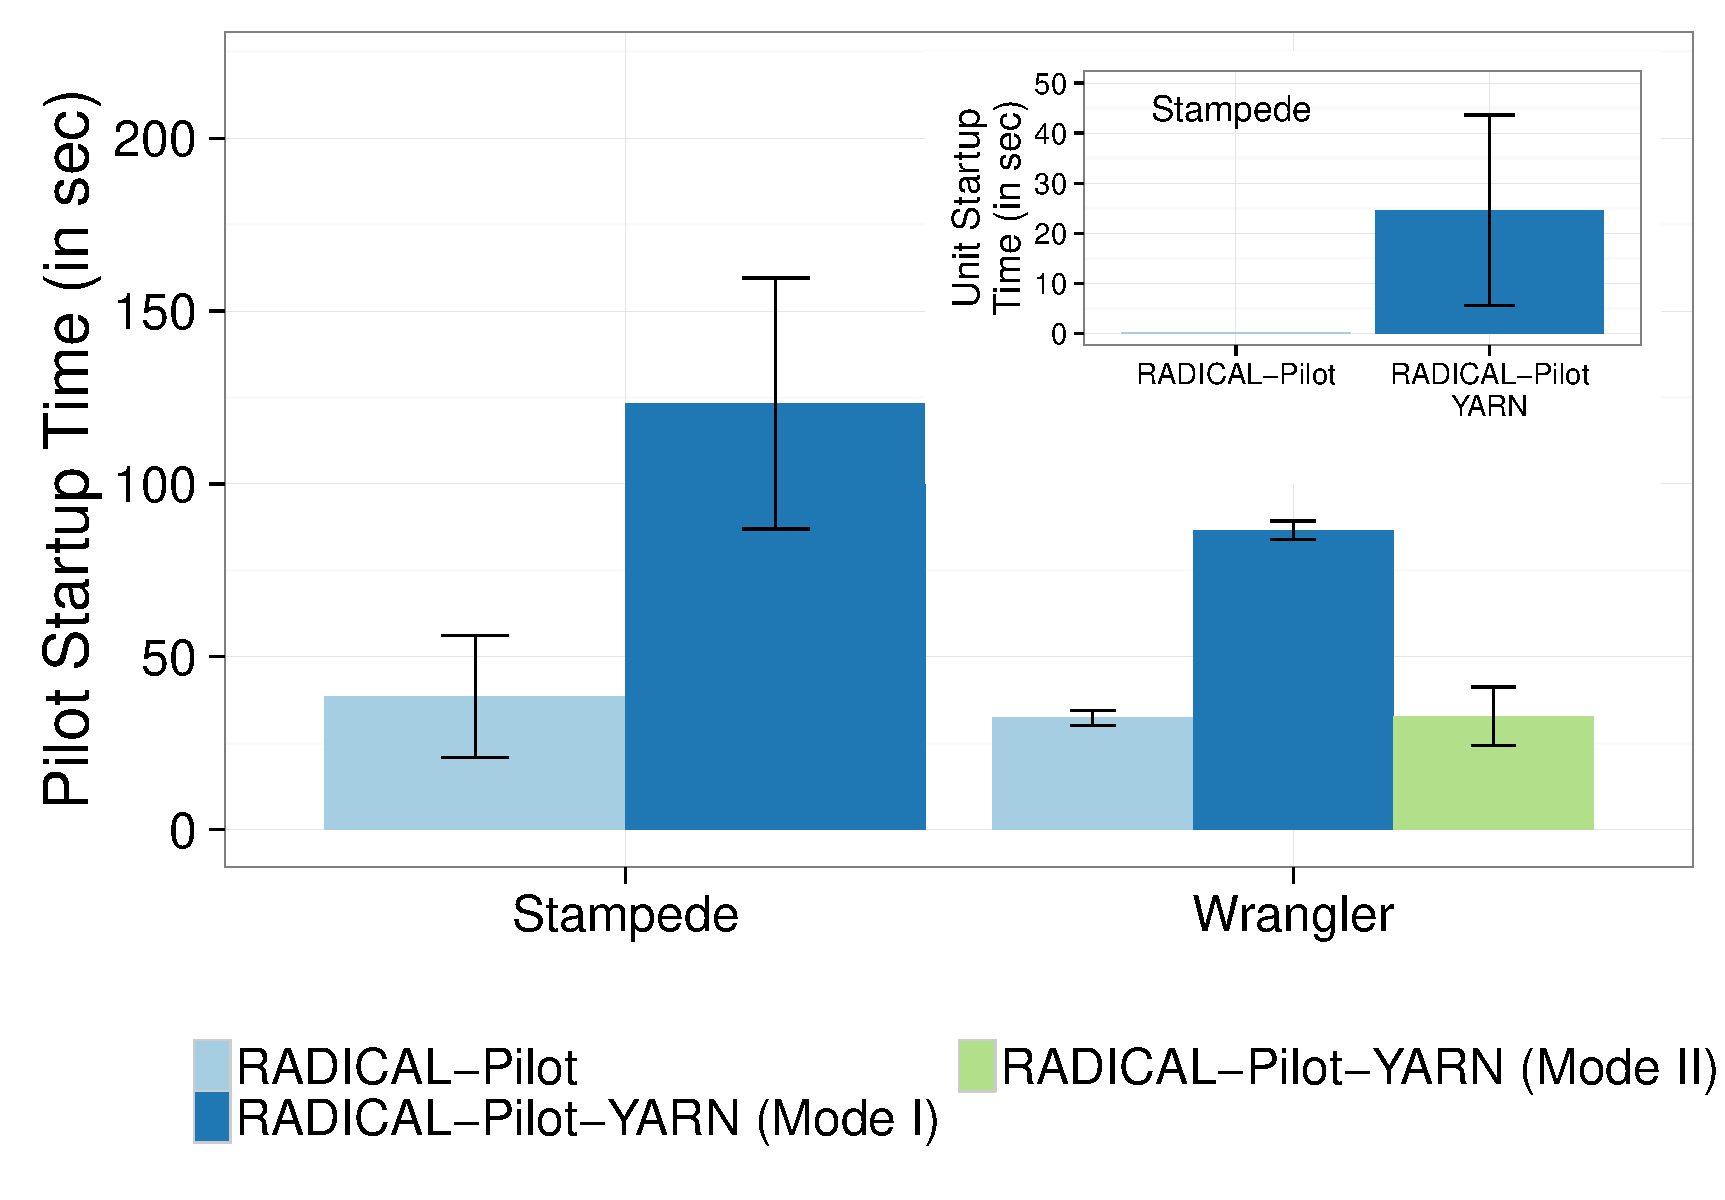
\includegraphics[width=0.75\textwidth]{figures/data_analytics_hpc/hpc_hadoop/pilot_unit_startup.pdf}
    \caption{RADICAL-Pilot and RADICAL-Pilot-YARN startup overheads.
        \label{fig:startup_yarn}}
%    \caption{\textbf{RADICAL-Pilot and RADICAL-Pilot-YARN startup overheads:}
%        The agent startup time is higher for YARN due to the overhead for spawning the YARN cluster.
%        The inset shows that the Compute Unit startup time (time between application submission to YARN and startup) is also significantly higher for YARN.
%        \label{fig:startup_yarn}}
\end{figure}

In Figure~\ref{fig:startup_yarn} we analyze the measured overheads when starting RADICAL-Pilot and RADICAL-Pilot-YARN, and when submitting Compute Units.
The agent startup time for RADICAL-Pilot-YARN is defined as the time between RADICAL-Pilot-Agent starts and the processing of the first Compute Unit.
On Wrangler, we compare both Mode I (Hadoop on HPC) and Mode II (HPC on Hadoop).
For Mode I the startup time is higher compared to the normal RADICAL-Pilot startup time and also compared to Mode II.
This can be explained by the necessary steps required tp download, configure and start the YARN cluster.
For a single node YARN environment, the overhead for Mode I (Hadoop on HPC) is between 50-85\,sec depending upon the resource selected.
The startup times for Mode II on Wrangler -- using the dedicated Hadoop environment provided via the data portal -- are comparable to the normal RADICAL-Pilot startup times as it is not necessary to spawn a Hadoop cluster.

The inset of Figure~\ref{fig:startup_yarn} shows the time taken to start Compute Units via RADICAL-Pilot to a YARN cluster.
For each CU, resources have to be requested in two stages: first the application master container is allocated followed by the containers for the actual compute tasks.
For short-running jobs this represents a bottleneck.

In summary, while there are overheads associated with executing inside of YARN, we believe these are acceptable, in particular for long-running tasks.
The novel capabilities of executing HPC tasks and YARN tasks within the same application has significant benefits for which measured overheads are likely acceptable.

\subsection{K-Means Performance Characterization}
\label{ssec:kmeans}
We compare the time to completion of the K-Means algorithm using two configurations: RADICAL-Pilot on HPC and RADICAL-Pilot in HPC/YARN mode. 
We use three different scenarios: 10,000 points and 5,000 clusters, 100,000 points / 500 clusters and 1,000,000 points / 50 clusters.
Each point belongs to a three dimensional space.
The compute requirements depend on the product of the number of points and clusters, thus it is constant for all three scenarios.
We use an optimized version of K-Means in which the sum and number of points are precomputed in the map phase, thus only these two attributes per cluster need to be shuffled.
The shuffle traffic depends on the number of clusters and decreases with the number of clusters.
For the purpose of this benchmark, we run two iterations of K-Means.

We utilize up to 3 nodes on Stampede and Wrangler.
Experiments are performed with the following configurations: 8 tasks on 1 node, 16 tasks on 2 nodes and 32 tasks on 3 nodes.
For RADICAL-Pilot-YARN, we use Mode II (Hadoop on HPC): the YARN Resource Manager is deployed on the node running the RADICAL-Pilot-Agent.

Figure~\ref{fig:experiments_kmeans_rpyarnkmeans} shows the results of executing K-Means over different scenarios and configurations.
For RADICAL-Pilot-YARN the runtimes include the time required to download and start the YARN cluster on the allocated resources.

\begin{figure}[t]
    \centering
    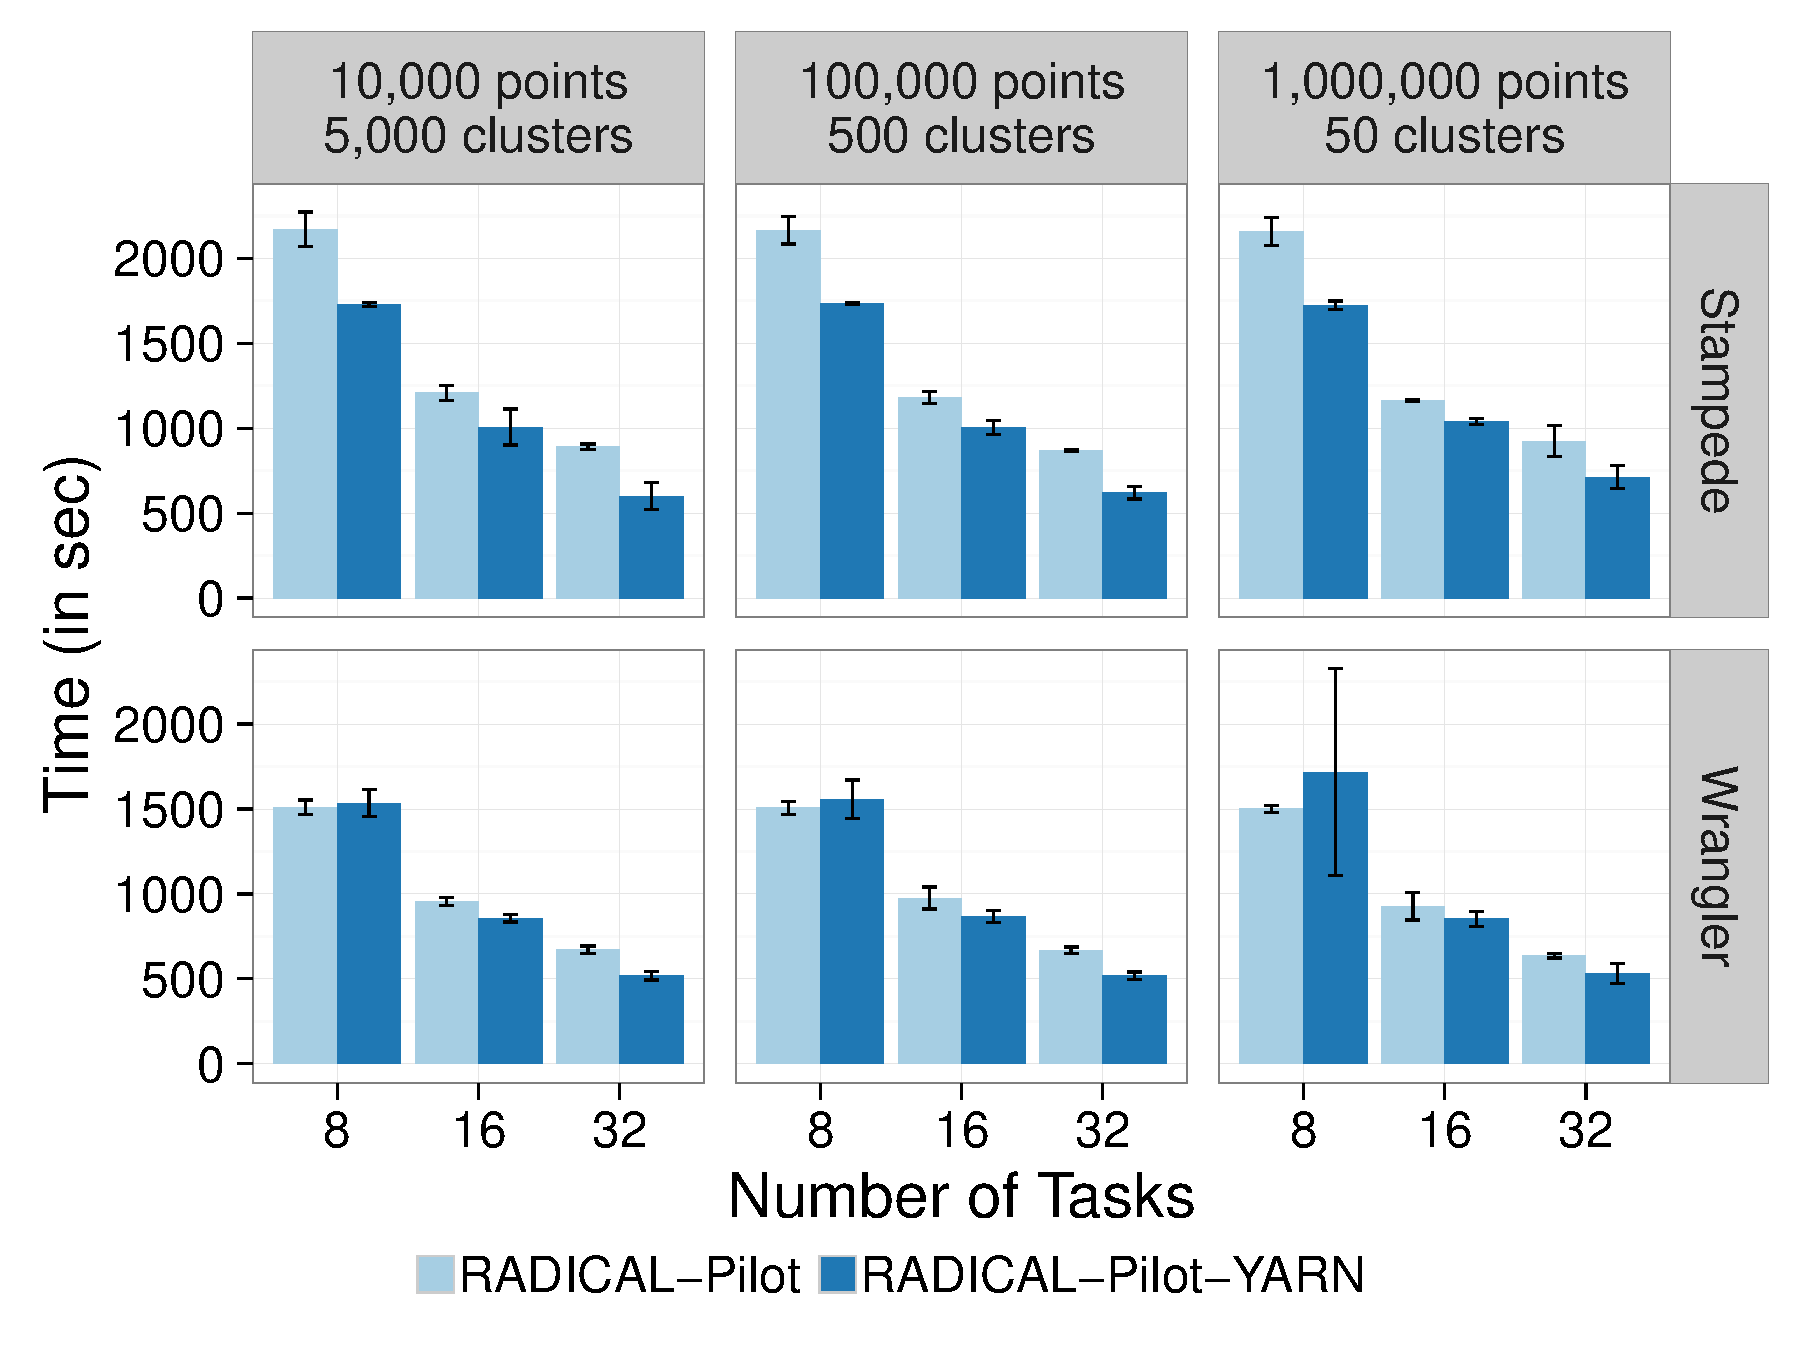
\includegraphics[width=.75\textwidth]{figures/data_analytics_hpc/hpc_hadoop/kmeans.pdf}
    \caption{RADICAL-Pilot and YARN-based K-Means time to completion on Stampede and Wrangler.}
%\caption{\textbf{RADICAL-Pilot and YARN-based K-Means on Stampede and Wrangler:}
%        Across all configurations the performance of the YARN backend is in average 13\,\% better.
%        On Wrangler a significant better performance and scalability (higher speedups) were observed.}
    \label{fig:experiments_kmeans_rpyarnkmeans}
\end{figure}

Independent of the scenario, the runtimes decrease with the number of tasks.
In particular, in the 8 task scenarios the overhead of YARN is visible on Wrangler.
For larger number of tasks, we observed on average 13~\% shorter runtimes for RADICAL-Pilot-YARN.
Also, RADICAL-Pilot-YARN achieves better speedups, e.\,g., 3.2 for 32 tasks for the 1 million points scenario, which is significantly higher than the RADICAL-Pilot speedup of 2.4 (both on Wrangler and compared to base case of 8 tasks).
One of the reasons is that for RADICAL-Pilot-YARN uses the local file system, while for RADICAL-Pilot uses the Lustre filesystem.

For similar scenarios and task/resource configuration, the runtimes on Wrangler show a significant performance improvements over Stampede.
This is attributed to the better hardware (CPUs, memory) of Wrangler than Stampede.
In particular for RADICAL-Pilot-YARN we observed on average higher speedups on Wrangler, indicating that we saturated the 32 GB of memory available on each Stampede node.

In summary, despite the overheads of RADICAL-Pilot-YARN with respect to Pilot and Compute Unit startup time, we were able to observe performance improvements (on average 13~\% better time to completion) mainly due to the better performance of the local disks.


\section{Conclusions}
\label{sec:hpc_hadoop_concl}
Hadoop and Spark are used by increasing number of scientific applications mainly due to accessible abstractions they provide.
HPC and Hadoop environments are converging, for example, MLLib/Spark utilize BLAS, Hadoop frameworks adopt parallel and in-memory computing concepts that originated in HPC.
Currently, traditional HPC applications lack the ability to access and use Hadoop and other Hadoop tools, without sacrificing the advantages of HPC environments.
One prominent reason behind the limited uptake, is finding effective and scalable resource management techniques usable for Hadoop frameworks on HPC infrastructure.

This chapter motivates the use of the Pilot-Abstraction as an integrating concept, discusses the design and implementation of RADICAL-Pilot extensions for Hadoop and Spark, and validates them with scalability analysis on two supercomputers.
Our experiments use RADICAL-Pilot, and introduce two extensions to RADICAL-Pilot to better integrate Hadoop on HPC.
We demonstrate that the Pilot-Abstraction strengthens the state of practice in utilizing HPC resources in conjunction with emerging Hadoop frameworks by allowing users to combine a diverse set of best-of-breed tools running on heterogeneous infrastructure consisting of HPC.
Using these capabilities, complex data campaigns can utilize a diverse set of Hadoop and HPC frameworks enabling scalable data ingests and analytics workflows.
Providing both a unifying and powerful abstraction that enables all parts of such a data pipeline to co-exist is critical.

While we demonstrated the importance of integrated capabilities for supporting data analytics on HPC, we want to understand their performance impact on scientific task-based data analytics scientific workflows.
This is important when executing computational campaigns on HPC resources, as selecting a suitable capability to execute data-intensive workflows is desirable.
Thus, we continue our work with integrating and measuring the performance of molecular dynamics data-analysis workflows utilizing these capabilities on HPC resources.

%%%%%%%%%%%%%%%%%%%%%%%%%%%%%%%%%%%%%%%%%%%%%%%%%%%%%%%%%%%%%%%%%%%%%%%%%%%%%%%%
%
%For example, Cray's analytics platform Urika~\footnote{http://www.cray.com/products/analytics} has Hadoop and Spark running on HPC architecture as opposed to regular clusters, but without the HPC software environment and capabilities.
%However, several applications ranging from bio-molecular simulations to epidemiology models~\cite{network1} require significant simulations interwoven with analysis capabilities such as clustering and graph analytics; in other words some stages (or parts of the same stage) of an application would ideally utilize Hadoop/Spark environments and other stages (or parts thereof) utilize HPC environments.
%
%Over the past decades, the High Performance Distributed Computing (HPDC) community has made significant advances in addressing resource and workload management on heterogeneous resources.
%For example, the concept of multi-level scheduling~\cite{1392910} as manifested in the decoupling of workload assignment from resource management using the concept of intermediate container jobs (also referred to as \pilotjobs~\cite{pstar12}) has been adopted for both HPC and Hadoop.
%Multi-level scheduling is a critical capability for data-intensive applications as often only application-level schedulers can be aware of the localities of the data sources used by a specific application.
%This motivated the extension of the \pilot-Abstraction to \pilotdata~\cite{pilot-data-jpdc-2014} to form the central component of a resource management middleware.
%
%In the following sections, we discuss a set of tools for supporting both of these usage modes:
%In section~\ref{ssec:saga_hadoop} we present SAGA-Hadoop, a light-weight tool for running Hadoop on HPC (Mode I).
%We then discuss, the integration of Hadoop and Spark runtimes into RADICAL-Pilot, which enables both the interoperable use of HPC and Hadoop, as well as the integration of HPC and Hadoop applications (Mode I and II) (Section~\ref{ssec:rp-impl}).
%Using these new capabilities, applications can seamlessly connect HPC stages (e.\,g.\ simulation stages) with analysis staging using the Pilot-Abstraction to provide unified resource management.
%
%\subsection{Mode I: SAGA-Hadoop, supporting Hadoop/Spark on HPC}
%\label{ssec:saga_hadoop}
%
%SAGA-Hadoop~\cite{saga-hadoop} is a tool for supporting the deployment of Hadoop and Spark on HPC resources (Mode I in Figure~\ref{fig:figures_hadoop-on-hpc-viceverse}).
%Using SAGA-Hadoop an applications written for YARN (e.\,g.\ MapReduce) or Spark (e.\,g. PySpark, DataFrame and MLlib applications) can be executed on HPC resources.
%
%Figure~\ref{fig:saga-hadoop} illustrates the architecture of SAGA-Hadoop.
%SAGA-Hadoop uses SAGA~\cite{merzky2015saga} to spawn and control Hadoop clusters inside an environment managed by an HPC scheduler.
%SAGA is used for dispatching a bootstrap process that generates the necessary configuration files and starting Hadoop.
%The specifics of the Hadoop framework (i.\,e.\ YARN and Spark) are encapsulated in a Hadoop framework plugin (also referred to as adaptors).
%SAGA-Hadoop delegates tasks, such as the download, configuration and start of a framework to this plugin.
%In the case of YARN, the plugin is then responsible for launching YARN's Resource and Node Manager processes; in the case of Spark, the Master and Worker processes.
%This architecture is extensible as new frameworks, e.\,g.\ Flink, can easily be added.
%
%\begin{figure}[t]
%    \centering
%    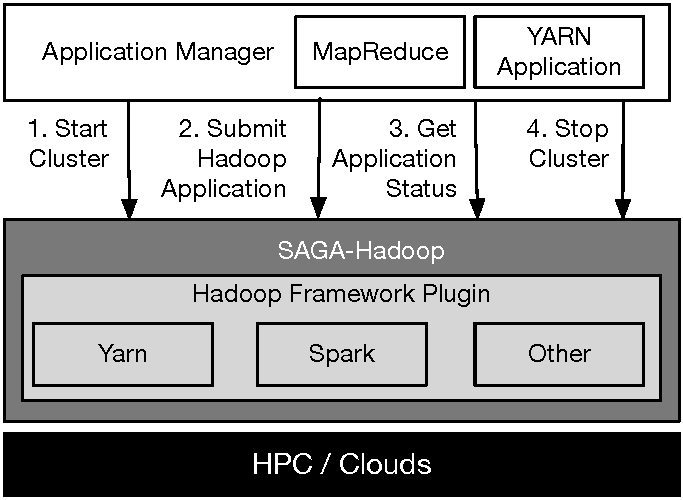
\includegraphics[width=.95\textwidth]{figures/data_analytics_hpc/hpc_hadoop/pilot-abds.pdf}
%    \caption{SAGA-Hadoop for HPC and Cloud Infrastructures.}
%    \label{fig:saga-hadoop}
%\end{figure}
%
%While nearly all Hadoop frameworks (e.\,g.\ MapReduce and Spark) support YARN for resource management, Spark provides a standalone cluster mode, which is more efficient in particular on dedicated resources.
%Thus, a special adaptor for Spark is provided.
%Once the cluster is setup, users can submit applications using SAGA's API that allows them to start and manage YARN or Spark application processes.
%
%While SAGA-Hadoop provides the interoperability between YARN and HPC resources by treating YARN as a substitute for common HPC schedulers, the integration of YARN and HPC applications or application stages remains challenging.
%As a consequence, we explored the usage of the Pilot~-Abstraction~\cite{luckow2012pstar}, through RADICAL-Pilot~\cite{merzky2019using}, to enable the integration between these different application types.


\section{Modeling the task-parallel execution of data intensive workflows}
\label{sec:task-par}

Data based workflow engines exploit task-parallelism by partitioning the data and generating stages of independent tasks.
These stages then ordered and implement data dependencies by shuffling, aggregating or coupling intermediate results.
The MapReduce~\cite{dean2004mapreduce} abstraction, along with its implementations, popularized this method of processing.

Spark~\cite{zaharia2010spark} and Dask~\cite{rocklin2015dask} are two Big Data frameworks.
Both provide MapReduce abstractions and are optimized for parallel processing of large data volumes, interactive analytics and machine learning.
Their runtime engines can automatically partition data, generate parallel tasks, and execute them on a cluster.
In addition, Spark offers in-memory capabilities allowing caching data that are read multiple times, making it suited for interactive analytics and iterative machine learning algorithms.
Dask also provides a MapReduce API (Dask Bags).
Furthermore, Dask's API is more versatile, allowing custom workflows and parallel vector/matrix computations.

\section{Molecular Dynamics (MD) Data Analysis}
%\label{ssec:use_cases}
Some commonly used algorithms for analyzing MD trajectories are Root Mean Square Deviation (RMSD), Pairwise Distances (PD), and Sub-setting~\cite{mura2014biomolecules}.
Two more advanced algorithms are Path Similarity Analysis (PSA)~\cite{seyler2015path} and Leaflet Identification~\cite{michaud2011mdanalysis}.
RMSD is used to identify the deviation of atom positions between frames.
PD and PSA methods calculate distances based on different metrics either between atoms or trajectories.
Sub-setting methods are used to isolate parts of interest of MD simulation.
Leaflet Identification provides information about groups of lipids by identifying the lipid leaflets in a lipid bilayer.
All these methods, in some way, read and process the whole physical system generated via simulations.
The analysis reduces the data to either a number or a matrix.

We discuss two of these methods, a Path Similarity Analysis (PSA) algorithm using the Hausdorff distance and a Leaflet Identification method, and their implementations in MDAnalysis~\cite{michaud2011mdanalysis,gowers2016mdanalysis}.
Section~\ref{ssec:mda} discusses the reasons for selecting these two algorithms in more detail.
%In addition, we implemented the PSA algorithm using CPPTraj~\cite{roe2013ptraj}.
%Furthermore, we explore the applications' Ogres Facets and Views~\cite{fox2014towards}, which provide a more systematic characterization.

%Big Data Ogres~\cite{fox2014towards} are organized into four classes, called \emph{views}.
%The possible features of a view are called \emph{facets}.
%A combination of facets from all views defines an Ogre.
%The Views are: 
%\begin{inparaenum}[1)]
%    \item execution - describes aspects, such as I/O, memory, compute ratios, whether computations are iterative, and the 5 V's of Big Data (Volume, Velocity, Value, Variety and Veracity),
%    \item data source \& style - discusses input data collection, storage and access,
%    \item processing - describes algorithms and kernels used for computation, and
%    \item problem architecture - describes the application architecture.
%\end{inparaenum}


\subsection{Applications and Algorithms: MDAnalysis}
\label{ssec:mda}
MDAnalysis is a Python library~\cite{michaud2011mdanalysis,gowers2016mdanalysis} that provides a comprehensive environment for filtering, transforming and analyzing MD trajectories in all commonly used file formats.
It provides a common object-oriented API to trajectory data and leverages existing libraries in the scientific Python software stack, such as NumPy~\cite{numpy} and Scipy~\cite{scipy}.

\subsubsection*{Path Similarity Analysis (PSA): Hausdorff Distance}Path Similarity Analysis (PSA)~\cite{seyler2015path} is used to quantify the similarity between trajectories considering their full atomic detail.
The basic idea is to compute pair-wise distances (for instance, using the Hausdorff metric~\cite{huttenlocher1993comparing}) between members of an ensemble of trajectories and cluster the trajectories based on their distance matrix.

Each trajectory is represented as a two dimensional array.
The first dimension corresponds to time frames of the trajectory, the second to the $N$ atom positions, in 3-dimensional space.

\begin{algorithm}[t]
    \scriptsize
    \caption{Path Similarity Algorithm: Hausdorff Distance}
    \label{alg:hausdorff}
    \begin{algorithmic}[1]
        \Procedure{HausdorffDistance}{$T_1$,$T_2$}\Comment{$T_1$ and $T_2$ are a set of 
            3D points}
        \State \texttt{List $D_1$,$D_2$}
        \For{$\forall frame_1$ in $T_1$}
        \For{$\forall frame_2$ in $T_2$}
        \State \texttt{Append in $D_1$ $d_{RMS}$($frame_1$, $frame_2$)}
        \EndFor
        \State \texttt{$D_{t_1}$ append $min(D_1)$}
        \EndFor
        \For{$\forall frame_2$ in $T_2$}
        \For{$\forall frame_1$ in $T_1$}
        \State \texttt{Append in $D_2$ $d_{RMS}$($frame_2$, $frame_1$)}
        \EndFor
        \State\texttt{$D_{t_2}$ append $min(D_2)$}
        \EndFor
        \State \textbf{return} $max\Big(max(D_{t_1}),max(D_{t_2})\Big)$
        \EndProcedure
        \\        
        \Procedure{PSA}{$Traj$}\Comment{$Traj$ is a set of trajectories}
        \For{$\forall T_1$ in $Traj$}
        \For{$\forall T_2$ in $Traj$}
        \State \texttt{ $D_{( T_1,T_2 )}$=HausdorffDistance$\Big( T_1,T_2 \Big)$} 
        \EndFor
        \EndFor
        \State \Return $D$
        \EndProcedure
    \end{algorithmic}
\end{algorithm}

Algorithm~\ref{alg:hausdorff} describes the PSA algorithm with the Hausdorff metric over multiple trajectories.
We apply a 2-dimensional data partitioning over the output matrix to parallelize, shown in algorithm~\ref{alg:partition}.
Our Hausdorff metric calculation is based on a naive algorithm.
Recently, an algorithm was introduced that uses early break to speedup execution~\cite{taha2015efficient}, although we are not aware of a parallel implementation of this algorithm.

\begin{algorithm}[t]
    \scriptsize
    \caption{Two Dimensional Partitioning}
    \label{alg:partition}
    \begin{algorithmic}[1]
        \State Initially, there are $N^2$ distances, where $N$ is the number of trajectories.
        Each distance defines a computation task.
        \State Map the initial set to a smaller set with $k=N/n_1$ elements, where $n_1$ is a divisor of $N$, by grouping $n_1$ by $n_1$ elements together.
        \State Execute over the new set with $k^2$ tasks.
        Each task is the comparisons between $n_1$ and $n_1$  elements of the initial set.
        They are executed serially.
    \end{algorithmic}
\end{algorithm}

The algorithm is embarrassingly parallel and uses linear algebra kernels for calculations.
It has complexity $O(n^2)$ (problem architecture \& processing views).
Input data volume is medium to large while the output is small.
Specific execution environments, such as HPC nodes, and Python arithmetic libraries, e.g., NumPy, are used (execution view).
Input data are produced by HPC simulations, and are stored on HPC storage systems, such as parallel filesystem like Lustre (data source \& style view).

Embarrassingly parallel algorithms are good candidates to utilize task parallelization.
The data are partitioned to independent parts and each part is assigned to a task.
These tasks can then execute as a bag of tasks.
As a result, they are ideally suited for task-management and MapReduce APIs.
They can be expressed as a bag of tasks using a task management API or a map-only application in a MapReduce-style API.
All three selected frameworks support the execution of bag of tasks, with RADICAL~-Pilot and Dask offering specific abstractions (as discussed in \S~\ref{ssec:frameworks}).

\subsubsection*{Leaflet Finder}Algorithm~\ref{alg:leafletfinder} describes the Leaflet Finder (LF) algorithm as presented in Ref.~\cite{michaud2011mdanalysis}.
LF assigns particles to one of two curved but locally approximately parallel sheets, provided that the inter-particle distance is smaller than the distance between sheets.
In biomolecular simulations of lipid membranes, consisting of a double layer of lipid molecules, LF is used to identify the lipids in the outer and inner leaflets (sheets).
The algorithm consists of two stages:
\begin{inparaenum}[a)]
    \item construction of a graph connecting particles based on threshold distance (cutoff), and
    \item computing the connected components of the graph, determining the lipids located on the outer and inner leaflets.
\end{inparaenum}

\begin{algorithm}[t]
    \scriptsize
    \caption{Leaflet Finder Algorithm}
    \label{alg:leafletfinder}
    \begin{algorithmic}[1]
        \Procedure{LeafletFinder}{$Atoms,Cutoff$}
        \Comment{$Atoms$ is a set of 3D points that represent the position of atoms in space. $Cutoff$ is an Integer Number}
        \State \texttt{Graph G =$(V=Atoms,E=\emptyset)$}
        \For{$\forall atom$ in $Atoms$}
        \State \texttt{$N = [a\in V: d(a,atom)\le Cutoff]$}
        \State \texttt{Add edges $[(atoms,a): a \in N]$ in G}
        \EndFor
        \State \texttt{C = ConnectedComponents(G)}
        \State \Return C
        \EndProcedure
    \end{algorithmic}
\end{algorithm}

The application stages have different complexities.
The first stage identifies neighboring atoms.
There are different implementation alternatives: 
\begin{inparaenum}[i)]
    \item computing the distance between all atoms ($O(n^2)$);
    \item utilizing a tree-based nearest neighbor (Construction: $O(n\log n)$, 
    Query: $O(\log n)$).
\end{inparaenum}
In both alternatives the input data volume is medium size and the output is smaller than the input.
The complexity of connected components is: $O(|V|+|E|)$ ($V$: Vertices, $E$: Edges), i.\,e. it greatly depends on the characteristics of the graph.

The application typically uses HPC nodes as the execution environment, and NumPy arrays (execution view).
It uses matrices to represent the physical system and the distance matrix.
The output data representation is a graph.
Leaflet Finder can be efficiently implemented using the MapReduce abstraction (problem architecture view).
It uses graph algorithms and linear algebra kernels (processing view facets).
The data source \& style view facets are the same as the PSA algorithm.

Leaflet Finder is more complex as it requires two stages.
It is possible to implement Leaflet Finder with a simple task-management API, although the MapReduce programming model allows more efficient implementation with a \texttt{map} for computing and filtering distances and a \texttt{reduce} for finding the components.
The shuffling required between map and reduce is medium as the number of edges is a fraction of the input data.
Spark and Dask natively support MapReduce and implementinf the Leaflet Finder algorithm is relatively straightforward.
RADICAL-Pilot, on the other hand, does not support natively MapReduce.
As a result, it is required by the application developer to define the data shuffling between the \emph{map} and \emph{reduce} phase of the algorithm.

%\subsubsection{CPPTraj}
%CPPTraj~\cite{roe2013ptraj,roe2018parallelization} is a C++ MD trajectory analysis tool.
%It is parallelized via MPI and OpenMP.
%CPPtraj reads in parallel frames from a single trajectory file or ensemble members of the same trajectory from different files.
%The frames are equally distributed to the MPI processes.
%Computational intensive algorithms are further parallelized using OpenMP.
%It requires at least one MPI process per ensemble member, where each member is a single trajectory file.


\subsection{Current Solutions for Parallel MD Data Analysis}
\label{ssec:related_work}
MD analysis algorithms were until recently executed serially and parallelization was not straightforward.
During the last years several frameworks emerged providing parallel algorithms for analyzing MD trajectories.
Some of those frameworks are CPPTraj~\cite{roe2013ptraj,roe2018parallelization}, HiMach~\cite{tiankai2008scalable}, PMDA~\cite{fan2019pmda}, Pteros 2.0~\cite{yesylevskyy2015pteros} and nMoldyn-3~\cite{hinsen2012nmoldyn}.
%We compare these frameworks with our approach over the parallelization techniques used.

Several different techniques are used for parallelizing these algorithms.
CPPTraj~\cite{roe2018parallelization} utilizes MPI and OpenMP to exeucte large scale analysis on HPC.
OpenMP is also utilized by Pteros~\cite{yesylevskyy2015pteros} to parallelize the compute intensive parts of the analysis.
HiMach~~\cite{tiankai2008scalable} extends Google's MapReduce and defines Map and Reduce methods.
nMoldyn-3~\cite{hinsen2012nmoldyn} parallelizes the execution through a Master Worker architecture.
The master defines analysis tasks, submits them to a task manager, which then are executed by the worker process.

%HiMach~\cite{tiankai2008scalable} was developed by D. E. Shaw Research group to provide a parallel analysis framework for MD simulations, and extends Google's MapReduce.
%HiMach API defines trajectories, does per frame data acquisition (Map) and cross-frame analysis (Reduce).
%HiMach's runtime is responsible to parallelize and distribute Map and Reduce phases to resources.
%Data transfers are done through a communication protocol created specifically for HiMach.

%Pteros-2.0~\cite{yesylevskyy2015pteros} is a open-source library that is used for modeling and analyzing MD trajectories, providing a plugin for each supported algorithm.
%The execution is done by a user defined driver application, which setups trajectory  I/O and frame dispatch for analysis.
%It offers a C++ and Python API.
%Pteros 2.0 parallelizes computational intensive algorithms via OpenMP and Multithreading.
%As a result, it is bounded to execute on a single node, making any analysis execution highly dependent on memory size.
%Through RADICAL-Pilot, Spark and Dask, we avoided recompiling every time there is a change to the underlying resource, ensuring the application's execution.

%MDTraj~\cite{mcgibbon2015mdtraj} is a Python package for analyzing MD trajectories.
%It links MD data and Python statistical and visualization software.
%MDTraj proposes parallelizing the execution by using the parallel package of IPython as a wrapper along with an out-of-core trajectory reading method.
%Our approach allows data parallelization on any level of the execution, not only in data read.

%nMoldyn-3~\cite{hinsen2012nmoldyn} parallelizes the execution through a Master Worker architecture.
%The master defines analysis tasks, submits them to a task manager, which then are executed by the worker process.
%In addition, it provides adaptability, allowing on-the-fly addition of resources, and execution fault tolerance when worker processes disconnect.

A common denominator of most approaches is that they do not use general purpose frameworks for parallelizing the execution.
Although, they are optimized to get as much performance as possible from the environments they are developed for, their portability is limited.
CPPTraj~\cite{roe2018parallelization} and Pteros~\cite{yesylevskyy2015pteros}, for example, are highly dependent on the underlying low level libraries of the resource they use.
HiMach~\cite{tiankai2008scalable} is build specifically for the Antons Supercomputer.

In contrast, our approach and PMDA~\cite{fan2019pmda} utilize more general purpose frameworks for parallelization.
Specifically, PMDA utilizes Dask to parallelize MD Trajectory analysis.
The frameworks used provide higher level abstractions, e.g machine learning, so any  integration with other data analysis methods can be fast and easier.
In addition, resource acquisition and management is done transparently.

\section{Task-Parallel Frameworks: RADICAL-Pilot, Spark, Dask}
\label{ssec:frameworks}
The landscape of frameworks for data-intensive applications is manifold~\cite{jha2014tale,kamburugamuve2017anatomy} and has been extensively studied in the context of scientific~\cite{jha2017introducing} applications.
In this section, we discuss the suitability of frameworks such as Spark~\cite{zaharia2010spark}, Dask~\cite{rocklin2015dask} and RADICAL~-Pilot~\cite{merzky2019using}, for MD data analytics.

\subsection{Background}
%MapReduce~\cite{dean2004mapreduce} and its open source Hadoop implementation combined a simple functional API with a powerful distributed computing engine that exploits data locality to allow optimized I/O performance.
%However, MapReduce is inefficient for interactive workloads and iterative machine learning algorithms~\cite{zaharia2010spark,ekanayake2010twister}.
Spark and Dask provide rich APIs, caching and other capabilities critical for analytics applications.
Spark is considered the standard solution for iterative data-parallel applications.
Dask is quickly gaining support in the scientific community, since it offers a fully python environment.
RADICAL~-Pilot is a Pilot-Job framework~\cite{luckow2012pstar} that supports task-level parallelism on HPC resources and adds a parallelization level on top of HPC MPI-based applications.
%RADICAL~-Pilot is a Pilot-Job framework~\cite{luckow2012pstar} that supports task-level parallelism on HPC resources.
%It successfully adds a parallelization level on top of HPC MPI-based applications.

As described in~\cite{jha2014tale}, these frameworks typically comprise of distinct layers, e.\,g.,cluster scheduler access, framework-level scheduling, and higher-level abstractions.
On top of low-level resource management capabilities various higher-level abstractions can be provided, e.\,g., MapReduce-inspired APIs.
These then provide the foundation for analytics abstractions, such as Dataframes, Datasets and Arrays.
Figure~\ref{fig:figures_bigdata_framework_stack} visualizes the different components of RADICAL~-Pilot, Spark and Dask.
The following describes each framework in detail.

\begin{figure}[ht]
    \centering
    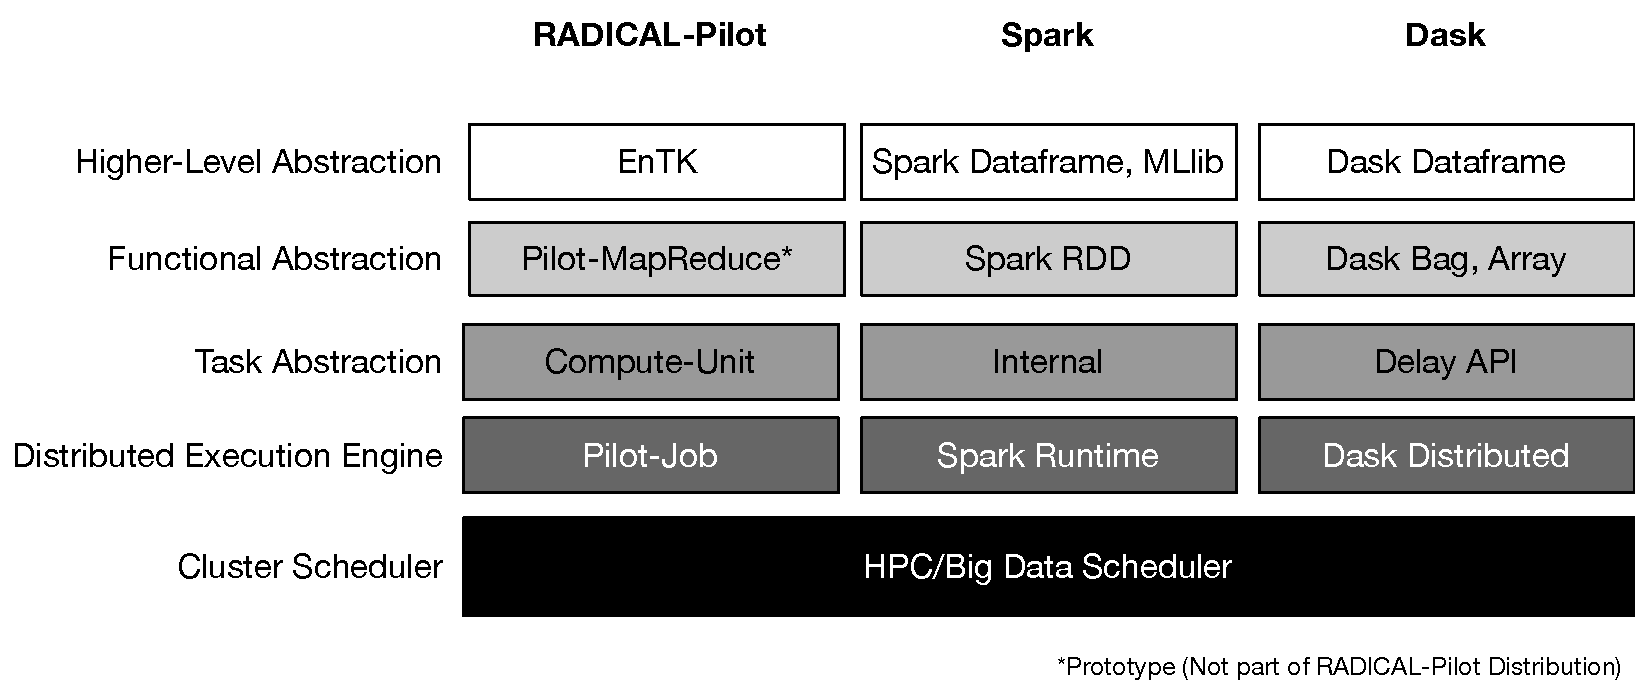
\includegraphics[width=.95\textwidth]{figures/data_analytics_hpc/task_par/bigdata_framework_stack.pdf}
    \caption{Architecture of RADICAL~-Pilot, Spark and Dask.}
    %\caption{\textbf{Architecture of RADICAL~-Pilot, Spark and Dask:}
    %The frameworks share common architectural components for managing cluster resource, and tasks.
    %Spark, Dask offer several high-level abstractions inspired by MapReduce.}
    \label{fig:figures_bigdata_framework_stack}
\end{figure}

\subsubsection*{RADICAL-Pilot}
%RADICAL~-Pilot~\cite{merzky2019using} is a Pilot system that implements the pilot paradigm as outlined in Ref.~\cite{turilli2018comprehensive}.
%RADICAL~-Pilot (RP) is implemented in Python and provides a well defined API and usage modes.
%Although RP is vehicle for research in scalable computing, it also supports production grade science.
%Currently, it is being used by applications drawn from diverse domains, ranging from earth and biomolecular sciences to high-energy physics.
%RP can be used as a runtime system by workflow or workload management systems~\cite{turilli2019middleware,treikalis2016repex,balasubramanian2018harnessing,dakka2018high,turilli2017evaluating}.
%In 2017, RP was used to support more than 100M core-hours on US DOE, NSF resources (BlueWaters and XSEDE), and European supercomputers (Archer and SuperMUC).

As discussed in \S~\ref{sec:pilot-data-hadoop}, RADICAL~-Pilot allows concurrent task execution on HPC resources.
The user defines a set of Compute~-Units (CU)~- the abstraction that defines a task along with its dependencies - which are submitted to RADICAL~-Pilot.
RADICAL~-Pilot schedules these CUs to be executed under the acquired resources.
It uses the existing environment of the resource to execute tasks.
Any data communication between tasks is done via an underlying shared filesystem, e.g., Lustre.
Task execution coordination and communication is done through a database (MongoDB).

%RADICAL~-Pilot's learning curve can be quite steep at the beginning, at least until the user becomes familiar with the concept and usability of Pilots and CUs.
%Once the user is comfortable with RADICAL~-Pilot's API, she can easily develop new algorithms.

\subsubsection*{Spark}
Spark~\cite{zaharia2010spark} extends MapReduce~\cite{dean2004mapreduce} providing a rich set of operations on top of the Resilient Distributed Dataset (RDD) abstraction~\cite{zaharia2012resilient}.
RDDs are cached in-memory making Spark well suitable for iterative applications that need to cache a set of data across multiple stages.
PySpark provides a Python API to Spark.

A Spark job is compiled of multiple stages; a stage is a set of parallel tasks executed without communicating (e.\,g., \texttt{map}) and an action (e.\,g., \texttt{reduce}).
Each action defines new stage.
The \texttt{DAGScheduler} is responsible for translating the workflow specified via RDD transformations and actions to an execution plan.
Spark's distributed execution engine handles the low-level details of task execution.
The execution of a Spark job is triggered by actions.
Spark can read data from different sources, such as HDFS, blob storage, parallel and local filesystems.
While Spark caches loaded data in memory, it offloads to disk when an executor does not have enough free memory to hold all the data of its partition.
Persisted RDDs remain in memory, unless specified to use the disk either complementary or as a single target.
In addition, Spark writes to disk data that are used in a shuffle.
As a result, it allows quick access to those data when transmitted to an executor.
Finally, Spark provides a set of actions that write text files, Hadoop sequence files or object files to local filesystems, HDFS or any filesystem that supports Hadoop.
In addition, Spark supports higher-level data abstractions for processing structured data, such as dataframes, Spark-SQL, datasets, and data streams.

\subsubsection*{Dask}
Dask~\cite{rocklin2015dask} provides a Python-based parallel computing library, which is designed to parallelize native Python code written for NumPy and Pandas.
In contrast to Spark, Dask also provides a lower-level task API (\texttt{delayed} API) that allows users to construct arbitrary workflow graphs.
Being written in Python, it does not require to translate data 
types from one language to another like PySpark, which moves data between Python's interpreter and Java/Scala.

In addition to the low-level task API, Dask offers three higher-level abstractions: Bags, Arrays and Dataframes.
Dask Arrays are a collection of NumPy arrays organized as a grid.
Dask Bags are similar to Spark RDDs and are used to analyze semi-structured data, like JSON files.
Dask Dataframe is a distributed collection of Pandas dataframes that can be analyzed in parallel.

Furthermore, Dask offers three schedulers: multithreading, multiprocessing and distributed.
The multithreaded and multiprocessing schedulers can be used only on a single node and the parallel execution is done via threads and processes respectively.
The distributed scheduler creates a cluster with a scheduling process and multiple worker processes.
A client process creates and communicates a DAG to the scheduler.
The scheduler assigns tasks to workers.

Dask's learning curve cannot be considered steep.
Its API is well defined and documented.
In addition, familiarity with Spark or MapReduce helps to minimize the learning curve even further.
As a result, implementing MD analysis algorithms on Dask did not require significant engineering time.
In addition, setting up a Dask cluster on a set of resources was relatively straightforward, since it provides all the binaries, e.g. \texttt(dask-ssh).

%\subsubsection*{RADICAL-Pilot}
%RADICAL~-Pilot~\cite{merzky2019using} is a Pilot system that implements the pilot paradigm as outlined in Ref.~\cite{turilli2018comprehensive}.
%RADICAL~-Pilot (RP) is implemented in Python and provides a well defined API and usage modes.
%Although RP is vehicle for research in scalable computing, it also supports production grade science.
%Currently, it is being used by applications drawn from diverse domains, ranging from earth and biomolecular sciences to high-energy physics.
%RP can be used as a runtime system by workflow or workload management systems~\cite{turilli2019middleware,treikalis2016repex,balasubramanian2018harnessing,dakka2018high,turilli2017evaluating}.
%In 2017, RP was used to support more than 100M core-hours on US DOE, NSF resources (BlueWaters and XSEDE), and European supercomputers (Archer and SuperMUC).

%RADICAL~-Pilot allows concurrent task execution on HPC resources.
%The user defines a set of Compute~-Units (CU)~- the abstraction that defines a task along with its dependencies - which are submitted to RADICAL~-Pilot.
%RADICAL~-Pilot schedules these CUs to be executed under the acquired resources.
%It uses the existing environment of the resource to execute tasks.
%Any data communication between tasks is done via an underlying shared filesystem, e.g., Lustre.
%Task execution coordination and communication is done through a database (MongoDB).

%RADICAL~-Pilot's learning curve can be quite steep at the beginning, at least until the user becomes familiar with the concept and usability of Pilots and CUs.
%Once the user is comfortable with RADICAL~-Pilot's API, she can easily develop new algorithms.

\subsection{Comparison}
\begin{table}[t]
    \begin{tabular}{@{}p{2.75cm}|p{3.25cm}p{3.25cm}p{3.25cm}@{}}
        \toprule
        &\textbf{RADICAL-Pilot} &
        \textbf{Spark} &
        \textbf{Dask} \\
        \midrule
        % row 1
        Languages &
        Python &
        Java, Scala, Python, R &
        Python\\
        % Row 2
        Task &
        Task &
        Map-Task &
        Delayed\\
        % row 3
        Abstraction &
        &
        & \\
        % row 4
        Functional Abstraction  &
        - &
        RDD API &
        Bag\\
        % row 5        
        Higher-Level Abstractions &
        EnTK~\cite{balasubramanian2018harnessing} &
        Dataframe, ML Pipeline, MLlib~\cite{meng2016mllib} &
        Dataframe, Arrays for block computations\\
        % row 6
        Resource Management &
        Pilot-Job &
        Spark Execution Engines &
        Dask Distributed Scheduler\\
        % row 7
        Scheduler    &
        Individual Tasks &
        Stage-oriented DAG &
        DAG\\
        % row 8        
        Shuffle      &
        -       &
        hash/sort-based shuffle &
        hash/sort-based shuffle\\
        % row 8
        Limitations &
        no shuffle, filesystem-based communication  &
        high overheads for Python tasks (serialization)   &
        Dask Array can not deal with dynamic output shapes\\
        \bottomrule
    \end{tabular}
    \caption{Task-parallel Frameworks Comparison.\label{tab:frameworks}}
    %\caption{\textbf{Task-parallel Frameworks Comparison:} Dask and Spark are designed for data-related task, while RADICAL~-Pilot focuses on compute-intensive tasks.\label{tab:frameworks}}
\end{table}

Table~\ref{tab:frameworks} summarizes the properties of these frameworks with respect to abstractions and runtime provided to create and execute parallel data applications. 

\subsubsection*{API and Abstractions} 
RADICAL~-Pilot provides a low-level API for executing tasks onto resources.
While this API can be used to implement high-level capabilities, e.\,g. MapReduce~\cite{mantha2012pilot}, they are not provided out-of-the box.
Both Spark and Dask provide such capabilities.
Dask's API is generally lower level than Spark's , e.\,g., it allows specifying arbitrary task graphs.
Although, data partition size is automatically decided, in many cases it is necessary to tune parallelism by specifying the number of partitions.

Another important aspect is the availability of high-level abstractions.
High-level tools for RADICAL~-Pilot, such as Ensemble Toolkit~\cite{balasubramanian2018harnessing}, are designed for workflows involving compute-intensive tasks.
Spark and Dask already offer a set of high-level data-oriented abstractions, such as Dataframes.

\subsubsection*{Scheduling}
Both Spark and Dask create a Direct Acyclic Graph (DAG) based on operations over data, which is then executed using their execution engine.
Spark jobs are separated into stages.
When a stage is completed, the scheduler executes the next stage.

Dask's DAGs are represented by a tree where each node is a task.
Leaf tasks do not depend on other task for execution.
Dask tasks are executed when their dependencies are satisfied, starting from leaf tasks.
When a task is reached with unsatisfied dependencies, the scheduler executes the dependent task first.
Dask's scheduler does not rely on synchronization points that Spark's stage-oriented scheduler introduces.
RADICAL~-Pilot does not provide a DAG and requires the execution order and synchronization to be specified by the user.

\subsection{Frameworks Evaluation}
\label{sec:framework_eval}

As data-parallelism often involves a large number of short-running tasks, task throughput is a critical metric to assess the different frameworks.
To evaluate the throughput we use zero workload tasks (\texttt{/bin/hostname}).
We submit an increasing number of such tasks to RADICAL~-Pilot, Spark and Dask and measure the execution time on a single node.

For RADICAL~-Pilot, all tasks were submitted simultaneously. RADICAL~-Pilot's backend database was running on the same node to avoid large communication latencies.
For Spark, we created an RDD with as many partitions as the number of tasks -- each partition is mapped to a task by Spark.
For Dask, we created tasks using \texttt{delayed} functions that were executed by the Distributed scheduler.
We used Wrangler and Comet for this experiment.

\begin{figure}[t]
    \centering
    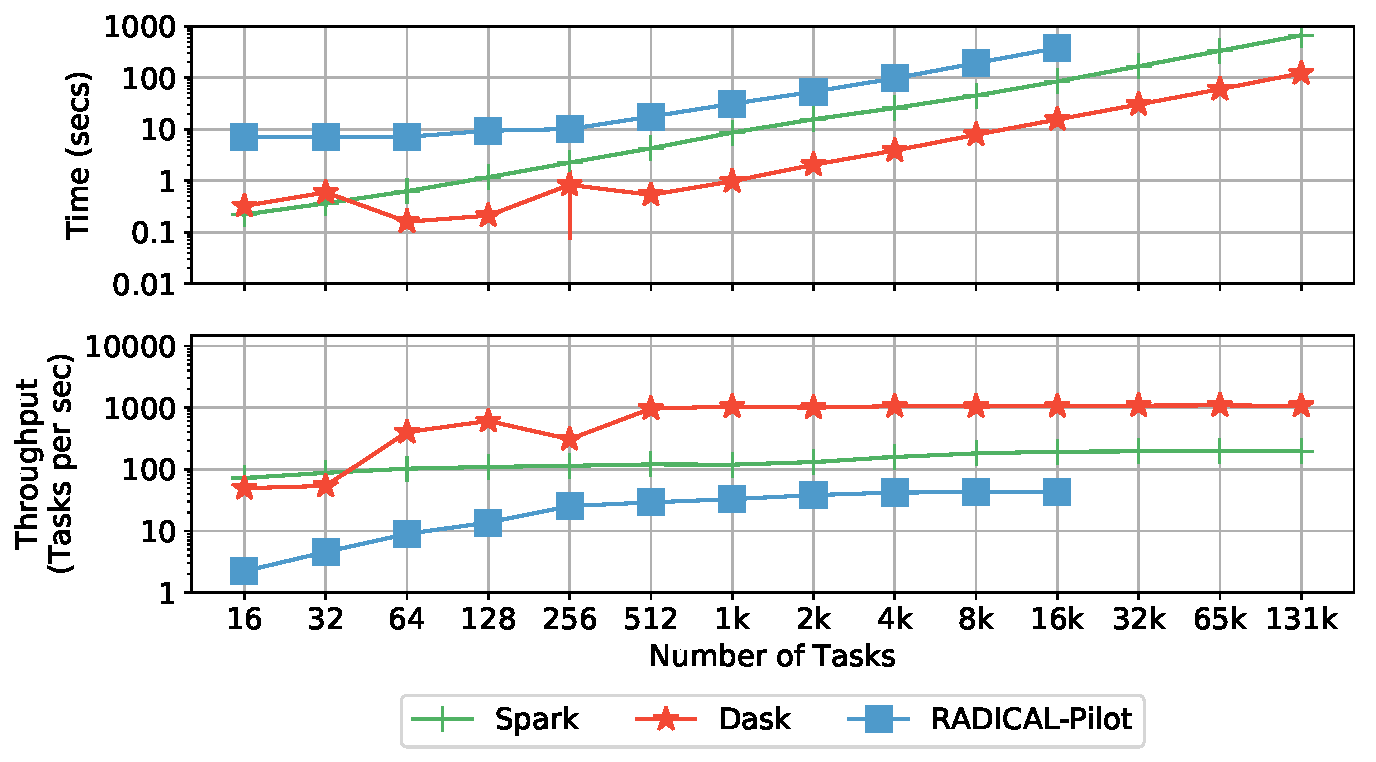
\includegraphics[width=.95\textwidth]{figures/data_analytics_hpc/task_par/dask_spark_rp_wrangler.pdf}
    \caption{Total time to completion and task throughput by framework on a single node for an increasing number of tasks.}
    %\caption{\textbf{Task Throughput by Framework (Single Node):} 
    %    Time/Throughput executing a given number of zero-workload tasks on Wrangler.
    %    Dask performs best; Dask and Spark have very small delays for few tasks.
    %    RADICAL~-Pilot offers the smallest throughput.}
    \label{fig:dask_spark_rp_wrangler}
\end{figure}

Figure~\ref{fig:dask_spark_rp_wrangler} shows the total time to completion and task throughput.
Dask needed the least time to schedule and execute the assigned tasks, followed by Spark and RADICAL~-Pilot.
Dask and Spark quickly reach their maximum throughput, which is sustained as the number of tasks increased.
RADICAL~-Pilot showed the worst throughput and scalability mainly due to some architectural limitations.
It relies on a MongoDB to communicate between Client and Agent, as well as several components that allow RADICAL~-Pilot to move data and introduce delays in the execution of the tasks.
Thus, we were not able to scale RADICAL~-Pilot to 32k or more tasks.

\begin{figure}[t]
    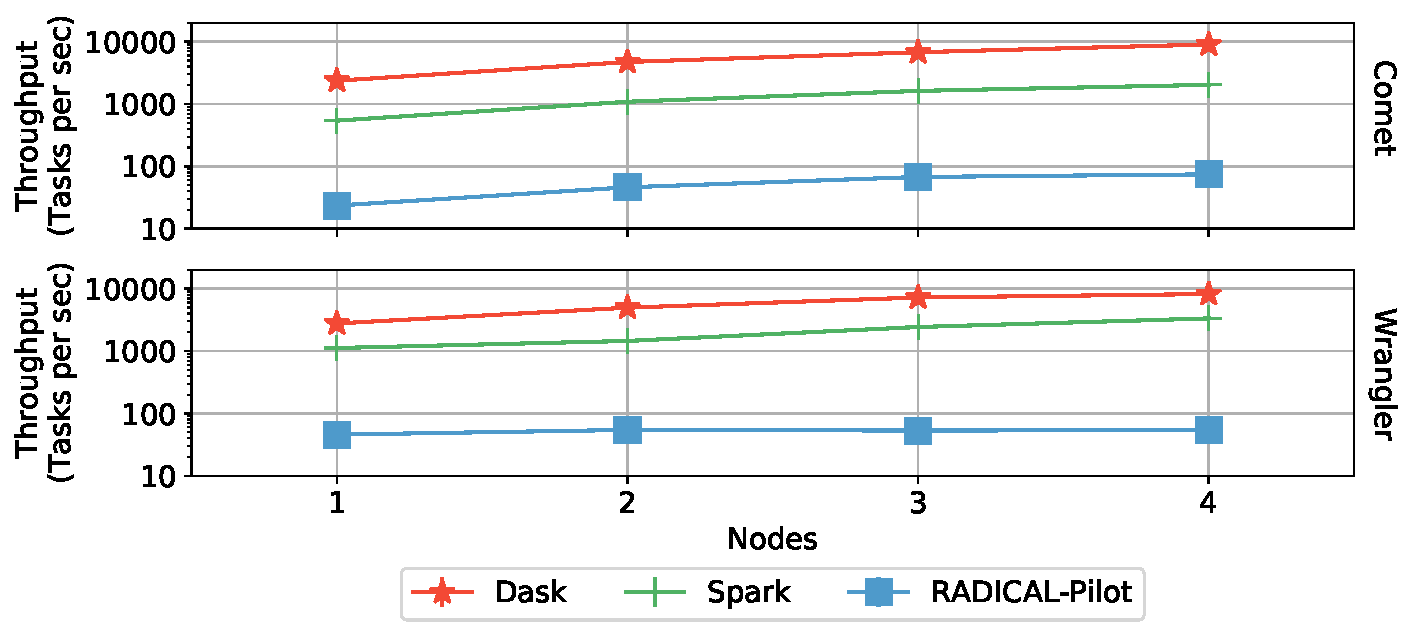
\includegraphics[width=.95\textwidth]{figures/data_analytics_hpc/task_par/daskVSsparkVSRpThroughput.pdf}
    \caption{Task throughput by framewrork for $100k$ tasks on different number of nodes.}
    %\caption{\textbf{Task Throughput by Framework (Multiple Nodes):}
    %    Task throughput for $100k$ zero-workload tasks on different numbers of nodes for each framework. 
    %    Dask has the largest throughput, followed by Spark and RADICAL~-Pilot.}
    \label{fig:RP_Dask_Spark_throughput}
\end{figure}

Figure~\ref{fig:RP_Dask_Spark_throughput} illustrates the throughput when scaling to multiple nodes measured by submitting $100k$ tasks.
Dask's throughput on both resources increases almost linearly to the number of nodes.
Spark's throughput is an order of magnitude lower than Dask's.
RADICAL~-Pilot's throughput plateaus at below $100 task/sec$.
Wrangler and Comet show a comparable performance with Comet slightly outperforming Wrangler.

%\subsubsection*{Suitability for MDAnalysis Algorithms}
%Trajectory analysis methods are often embarrassingly parallel.
%So, they are ideally suited for task management and MapReduce APIs.
%PSA-like methods typically require a single pass over the data and return a set of values that correspond to a relationship between frames or trajectories.
%They can be expressed as a bag of tasks using a task management API or a map-only application in a MapReduce-style API.

%Leaflet Finder is more complex and requires two stages:
%\begin{inparaenum}[a)]
%    \item the edge discovery stage, and
%    \item the connected components stage.
%\end{inparaenum}
%It is possible to implement Leaflet Finder with a simple task-management API, although the MapReduce programming model allows more efficient implementation with a \texttt{map} for computing and filtering distances and a \texttt{reduce} for finding the components.
%The shuffling required between map and reduce is medium as the number of edges is a fraction of the input data.

\section{Task-Parallel MD Trajectory Data Analysis: Implementation \& Characterization}
\label{impl_exp}
In this section, we characterize the performance of RADICAL~-Pilot, Spark and Dask compared to MPI4py.
In section~\ref{sec:framework_eval} we evaluate the task throughput using a synthetic workload.
In sections~\ref{sec:psa} and~\ref{sec:leaflet} we evaluate the performance of two algorithms from MDAnalysis: PSA and Leaflet Finder using different real-world datasets.
We investigate: 
\begin{inparaenum}[1)]
    \item which capabilities and abstractions of the frameworks are needed to efficiently express these algorithms,
    \item what architectural approaches can be used to implement these algorithms with these frameworks, and
    \item the performance trade-offs of these frameworks.
\end{inparaenum}

The experiments were executed on the XSEDE Supercomputers: Comet and Wrangler.
SDSC Comet is a 2.7 PFlop/s cluster with 24\, Haswell cores/node and 128\,GB memory/node (6,400 nodes).
TACC Wrangler has 24\, Haswell hyper-threading enabled cores/node and 128\,GB memory/node (120 nodes).
Experiments were carried using RADICAL~-Pilot and Pilot-Spark (as discusses on \S~\ref{sec:pilot-data-hadoop}) extension, which allows to efficiently manage Spark on HPC resources through a common resource management API.
We utilize a set of custom scripts to start the Dask cluster.
We used RADICAL~-Pilot 0.46.3, Spark 2.2.0, Dask 0.14.1 and Distributed 1.16.3.
The data presented are means over multiple runs; error bars represent the standard deviation of the sample.
We employed up to $10$ nodes in Comet and Wrangler. 

\subsection{Path Similarity Analysis: Hausdorff Distance}
\label{sec:psa}
The PSA algorithm is embarrassingly parallel and can be implemented using simple task-level parallelism or a map only MapReduce application.
The input data, i.\,e. a set of trajectory files, is equally distributed over the cores, generating one task per core.
Each task reads its respective input files in parallel, executes and writes the result to a file.

For RADICAL~-Pilot we define a Compute~-Unit for each task and execute them using a Pilot-Job. 
For Spark, we create an RDD with one partition per task.
The tasks are executed in a \texttt{map} function.
In Dask, the tasks are defined as \texttt{delayed} functions.
In MPI, each task is executed by a process.

The experiments were executed on Comet and Wrangler. 
The dataset used consists of three different atom count trajectories: 
\begin{inparaenum}[1)]
    \item small ($3341$ atoms/frame), 
    \item medium ($6682$ atoms/frame) and 
    \item large ($13364$ atoms/frame).
\end{inparaenum}
We used $102$ frames, and $128$ and $256$ trajectories of each size.

Figure~\ref{fig:HausdorffWrangler} shows the runtime for 128 and 256 trajectories on Wrangler.
Figure~\ref{fig:comet_wrangler_haus} compares the execution times on Comet and Wrangler for $128$ large trajectories.
We see that the frameworks have similar performance on both systems.
Furthermore, we see that Wrangler gives smaller speedup than Comet.
Although, we used the same number of cores, we see that utilizing half the nodes due to hyperthreading results to smaller speedup.

\begin{figure}[t]
    \centering
    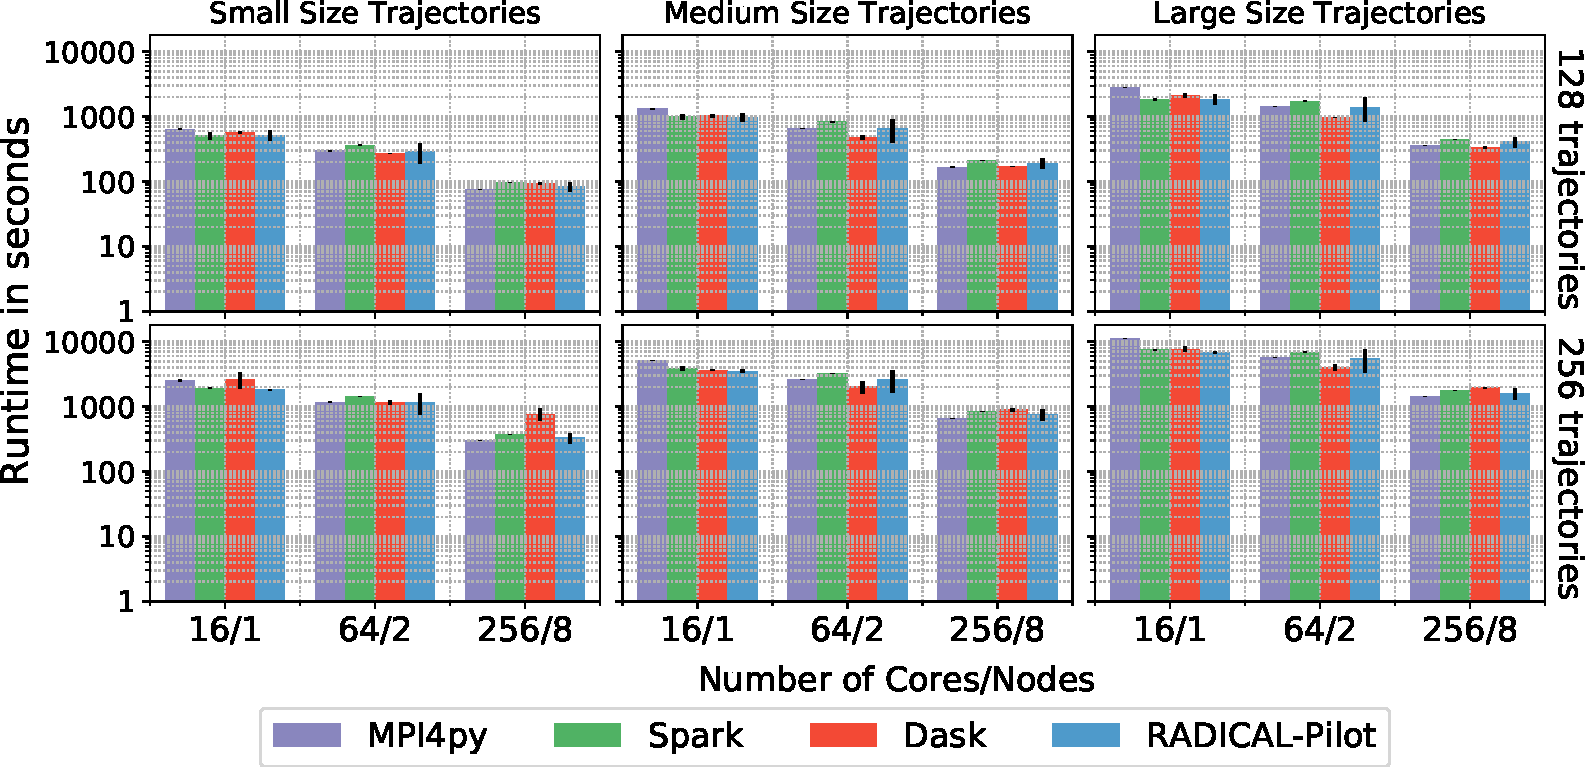
\includegraphics[width=0.95\textwidth]{figures/data_analytics_hpc/task_par/HausdorffSingleFig.pdf}
    \caption{Time to completion of Hausdorff Distance on Wrangler using RADICAL~-Pilot, Spark and Dask over different number of cores, trajectory sizes, and number of trajectories.}
%    \caption{\textbf{Hausdorff Distance on Wrangler using RADICAL~-Pilot, Spark and Dask:}
%            Runtimes over different number of cores, trajectory sizes, and number of trajectories.
%            All frameworks scaled by a factor of 6 from 16 to 256 cores.}
            \label{fig:HausdorffWrangler}
\end{figure}

\begin{figure}[t]
    \centering
    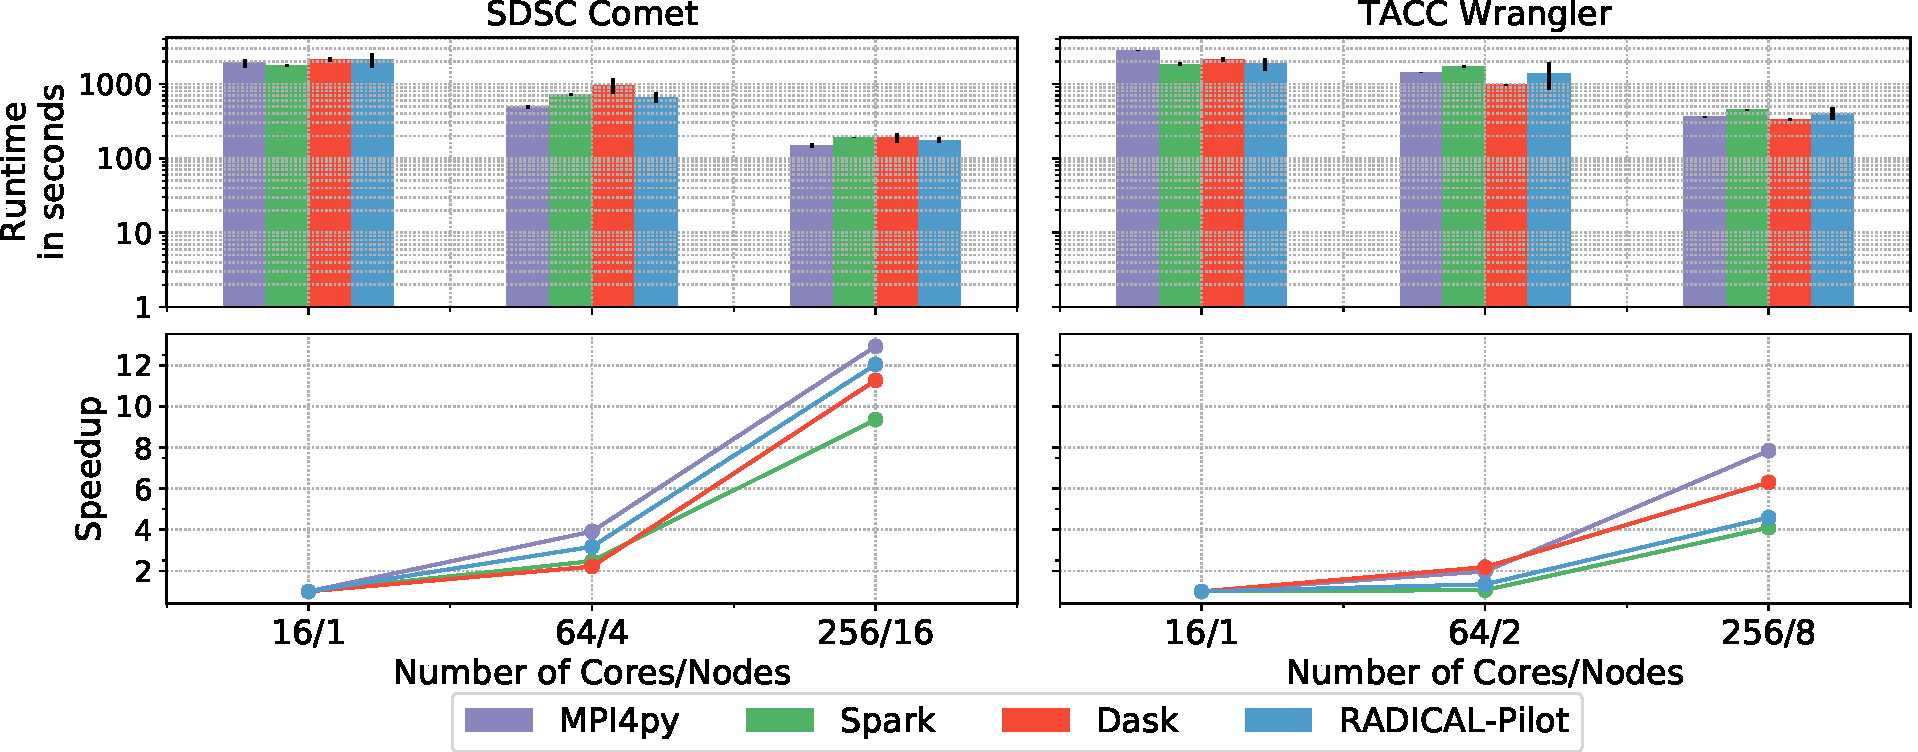
\includegraphics[width=.95\textwidth]{figures/data_analytics_hpc/task_par/comet_wrangler_haus.pdf}
    \caption{Time to completion and speedup of Hausdorff Distance execution on Comet and Wrangler for 128 large trajectories.} 
    \label{fig:comet_wrangler_haus}
\end{figure}

MPI4py, RADICAL~-Pilot, Spark and Dask have similar performance when used to execute embarrassingly parallel algorithms.
All frameworks achieved similar speedups as the number of cores increased, scaling by a factor of 6 from 16 to 256 cores, which are lower than MPI4py.
Although, the frameworks' overheads are comparably low in relation to the overall runtime, they were significant to impact their speedup.
RADICAL~-Pilot's large deviation is due to sensitivity to communication delays with the database.
In summary, all three frameworks provide appropriate abstractions and runtime performance, compared to MPI, for embarrassingly parallel algorithms. 
In this case aspects such as programmability and integrate-ability are more important considerations,e.\,g., both RADICAL~-Pilot and Dask are native Python frameworks making the integration with python native frameworks easier and more efficient than with other frameworks, which are based on other languages.

%\begin{figure}[ht]
%    \centering
%    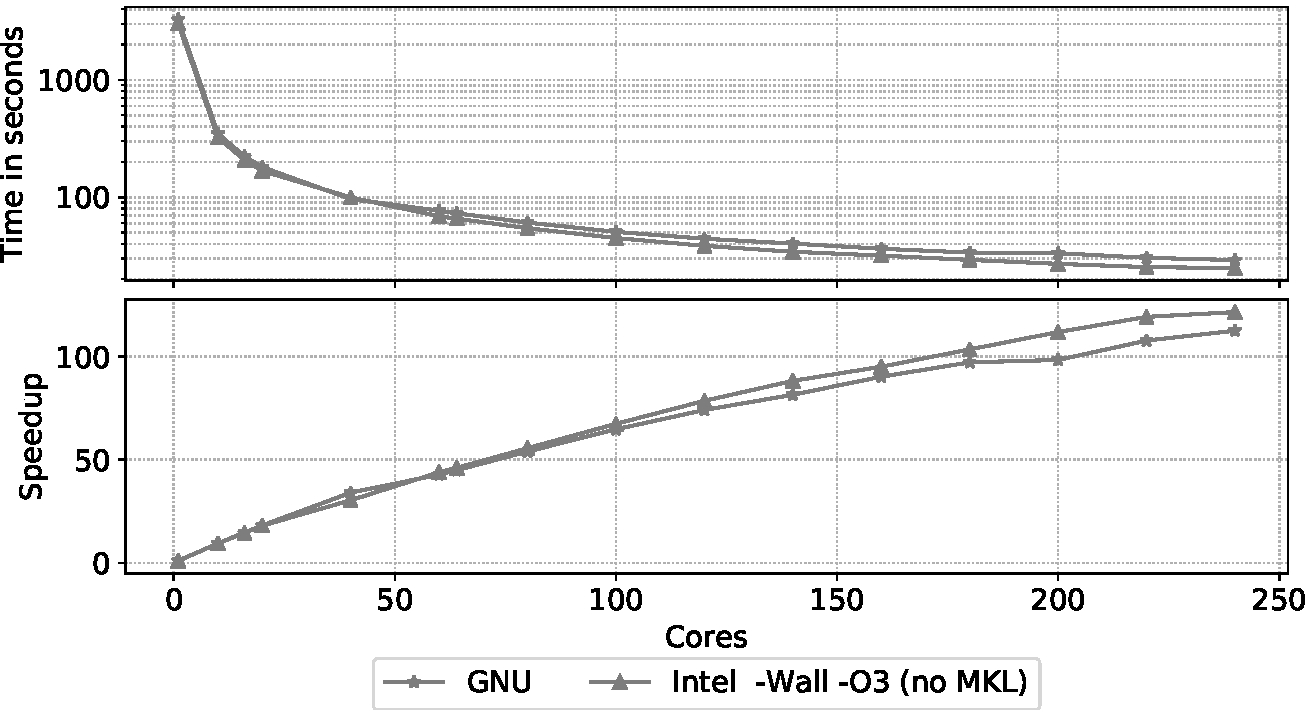
\includegraphics[width=.95\textwidth]{figures/data_analytics_hpc/task_par/cpptrajHausdorff.pdf}
%    \caption{\label{fig:cpptraj_resutls}\textbf{Hausdorff Distance using CPPTraj:}
%    Runtimes and Speedup over different number of cores.} 
%\end{figure}

%CPPTraj~\cite{roe2018parallelization} provides an optimized C++ implementation of the 2D-RMSD, which is Algorithm~\ref{alg:hausdorff} with no $\min-\max$ operations.
%The 2D-RMSD between trajectories was executed in parallel.
%The results were gathered and the Hausdorff distance was calculated.
%CPPTraj~\cite{roe2018parallelization} was compiled with GNU C++ compiler and no optimizations, and with Intel's compiler O3 optimization enabled.
%An experiment was run with 20-core Haswell nodes and 128 small trajectories; number of cores ranging from 1 up to 240.
%Figure~\ref{fig:cpptraj_resutls} shows the runtimes and speedup.
%MPI C++ provides lower execution times.
%However, we are interested in scalable solutions, that may offer worse performance in absolute numbers, but allows easier integration, i.e., less lines of code, and/or less engineering time.

\subsection{Leaflet Finder}
\label{sec:leaflet}
\begin{table*}[t]
    \centering
    \begin{tabular}{@{}p{2cm}|p{2.8cm}p{2.8cm}p{2.8cm}p{2.8cm}@{}}
        \toprule
        &
        \textbf{Broadcast and 1-D} (Approach 1) &
        \textbf{Task API and 2-D} (Approach 2) &
        \textbf{Parallel Connected Components} (Approach 3) &
        \textbf{Tree-Search} (Approach 4)\\
        \midrule
        % row 1
        Data Partitioning  & 
        1D  & 
        2D & 
        2D & 
        2D\\
        % row 2
        Map & 
        Edge Discovery via Pairwise Distance &
        Edge Discovery via Pairwise Distance &
        Edge Discovery via Pairwise Distance and Partial Connected Components & 
        Edge Discovery via Tree-based Algorithm and Partial Connected Components\\
        % row 3
        Shuffle &
        Edge List ($O(E)$) &
        Edge List ($O(E)$) &
        Partial Connected components ($O(n)$) &
        Partial Connected components ($O(n)$)\\
        % row 4
        Reduce   &
        Connect Components  &
        Connected Components &
        Joined Connected Components &
        Joined Connected Components\\
        \bottomrule
    \end{tabular}
    \caption{MapReduce Operations used by Leaflet Finder\label{tab:app_operators}}
\end{table*}

\begin{figure*}[t]
    \centering
    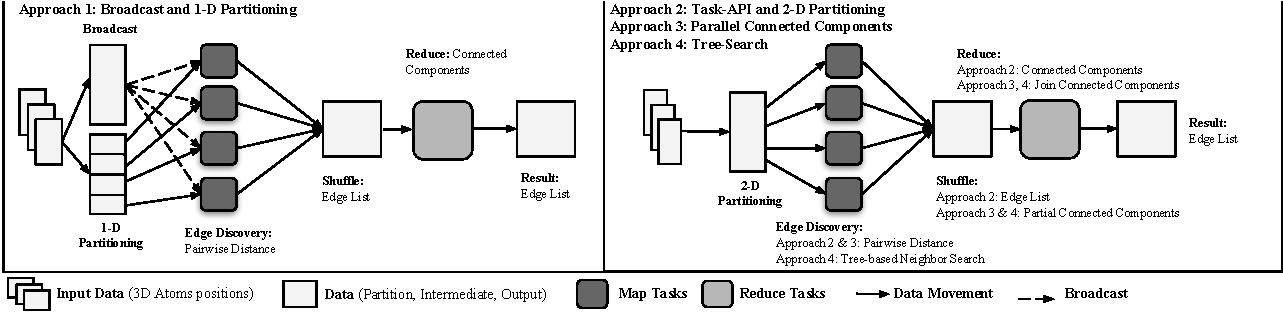
\includegraphics[width=.98\textwidth]{figures/data_analytics_hpc/task_par/lf_approaches.pdf}
    \caption{Architectural approaches for implementing the Leaflet finder algorithm\label{fig:lf_approaches}} 
\end{figure*}

We developed four different approaches for implementing the Leaflet Finder algorithm using RADICAL~-Pilot, Spark, Dask, and MPI4py (see Fig~\ref{fig:lf_approaches} and Table~\ref{tab:app_operators}):
\begin{enumerate}[1)]
    \item \textbf{Broadcast and 1-D Partitioning:}
    The physical system is broadcast and partitioned through a data abstraction.
    Use of RDD API (broadcast), Dask Bag API (scatter), and MPI Bcast to distribute data to all nodes.
    A \texttt{map} function calculates the edge list using \texttt{cdist} from SciPy~\cite{scipy} -- realized as a loop for MPI.
    The list is collected to the master process (gathered to rank 0) and the connected components are calculated.\label{en:1}
    \item \textbf{Task API and 2-D Partitioning:}
    Data management is done without using the data-parallel API.
    The framework is used for task scheduling.
    Data are pre-partitioned in 2-D partitions and passed to a \texttt{map} function that calculates the edge list using \texttt{cdist}-- realized as a loop for MPI.
    The list is collected (gathered to rank 0) and the connected components are calculated.\label{en:2}
    \item \textbf{Parallel Connected Components:}
    Data are managed as in approach~\ref{en:2}.
    Each \texttt{map} task performs edge list and connected components computations.
    The reduce phase joins the calculated components into one, when there is at least one common node.\label{en:3}
    \item \textbf{Tree-based Nearest Neighbor and Parallel-Connected Components (Tree-Search):}
    This approach is different to approach~\ref{en:3} only on the way edge discovery in the \texttt{map} phase is implemented.
    A tree containing all atoms is created which is then used to query for adjacent atoms.\label{en:4}
\end{enumerate}

We use four physical systems with $131k$, $262k$, $524k$, and $4M$ atoms with $896k$, $1.75M$, $3.52M$, and $44.6M$ edges in their graphs.
Experimentation was conducted on Wrangler where we utilized up to 256 cores.
Data partitioning results into $1024$ partitions for each approach, thus $1024$ \texttt{map} tasks.
Due to memory limitations from using \texttt{cdist} -- uses double precision floating point -- Approach \ref{en:3} data partitioning of the $4M$ atom dataset resulted to $42k$ tasks for both Spark and MPI4py.

Figure \ref{fig:All4approachesNoRp} shows the runtimes for all datasets for Spark, Dask and MPI4py.
RADICAL~-Pilot's performance is illustrated in Figure~\ref{fig:rpLF}.
We continue by analyzing the performance of each architectural approach and used framework in detail.

\begin{figure}[t]
    \begin{subfigure}{.95\textwidth}
        \centering
        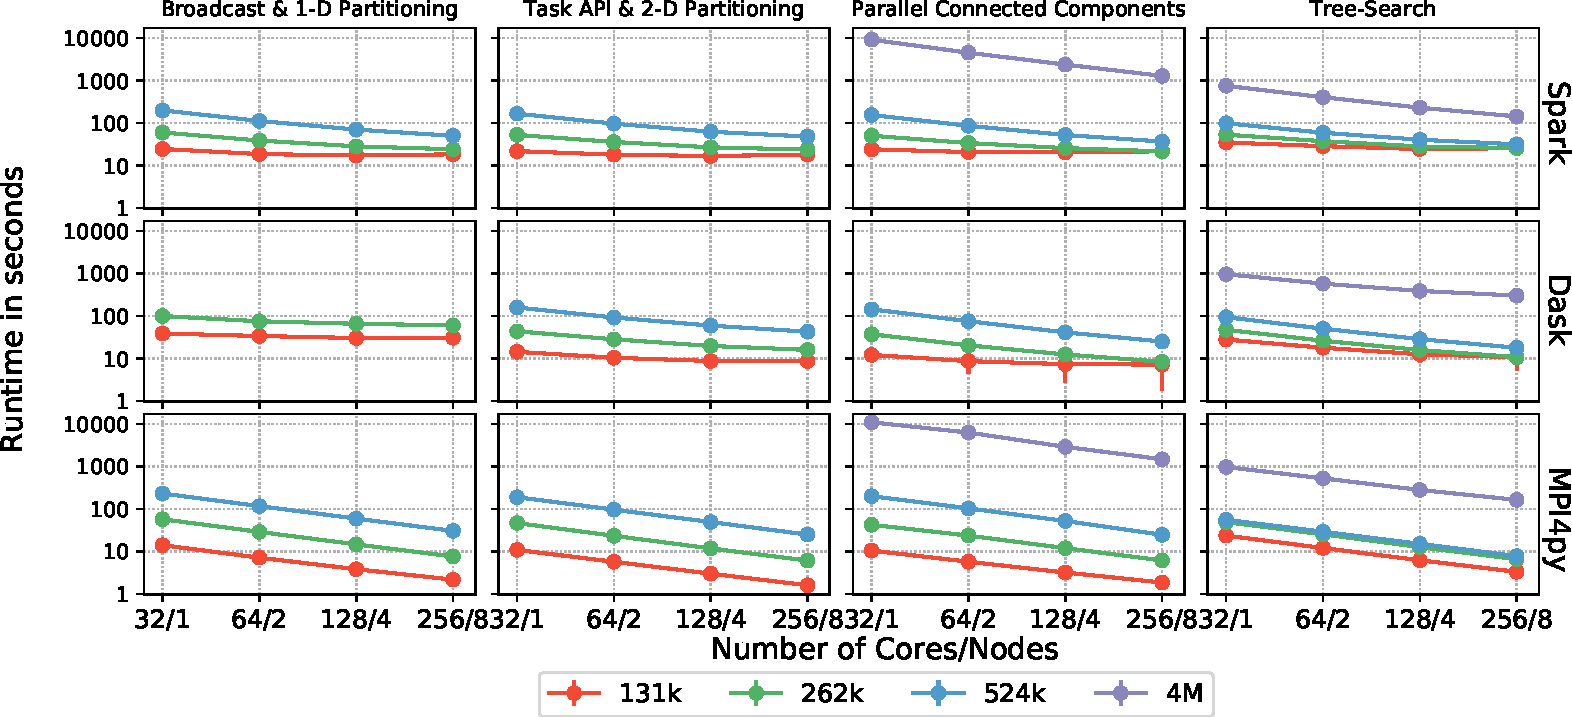
\includegraphics[width=1\linewidth]{figures/data_analytics_hpc/task_par/All4approachesWith4M_logscaleline.pdf}
    \end{subfigure}\\
    \begin{subfigure}{.95\textwidth}
        \centering
        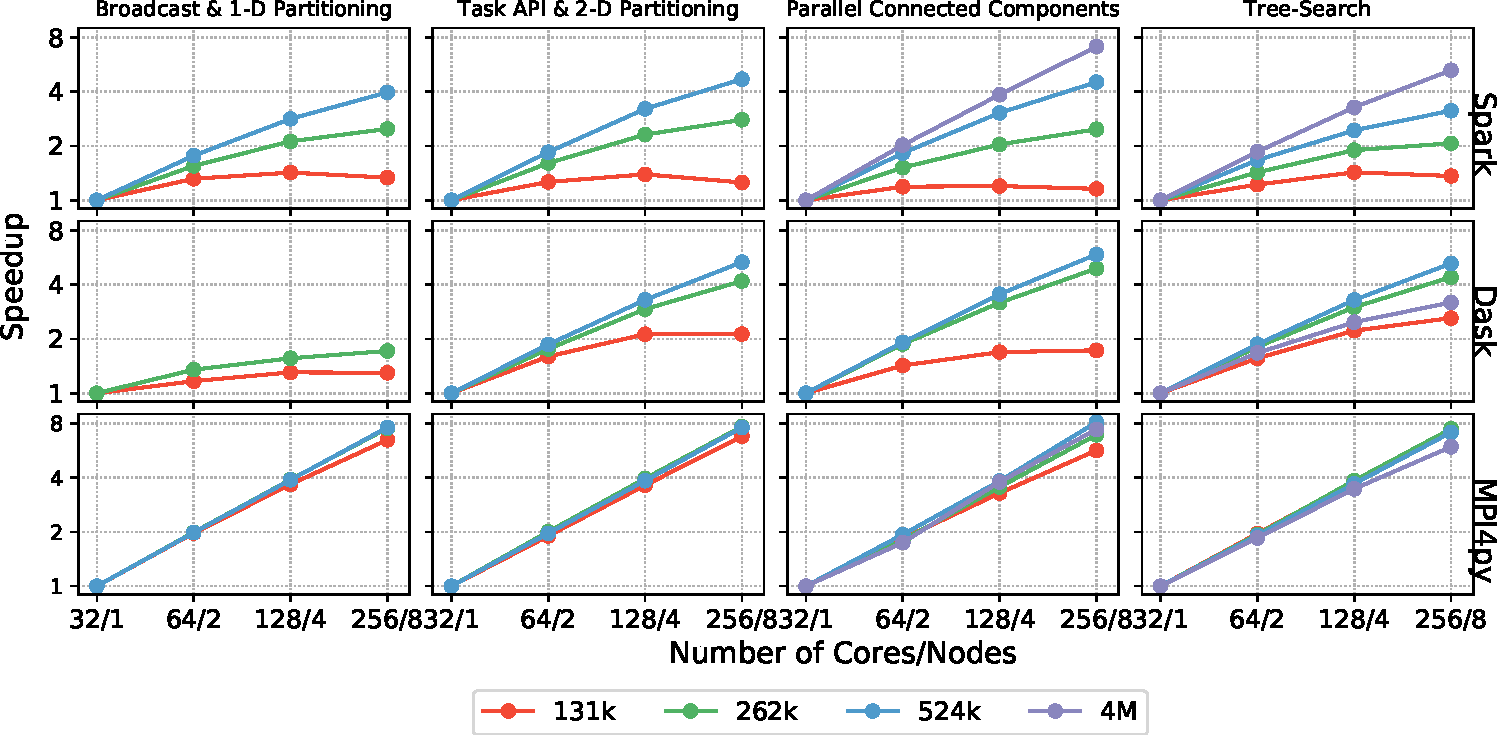
\includegraphics[width=.95\linewidth]{figures/data_analytics_hpc/task_par/All4approachesWith4MSpeedup.pdf}
    \end{subfigure}
    \caption{Leaflet Finder Performance of Different Architectural Approaches for Spark \& Dask.
            Runtimes and Speedups for different system sizes over different number of cores for all approaches and frameworks.}
    \label{fig:All4approachesNoRp}
\end{figure}

%%%%%%%%%%%%%%% APPROACH 1 %%%%%%%%%%%%%%%%%%

\begin{figure}[t]
    \centering
    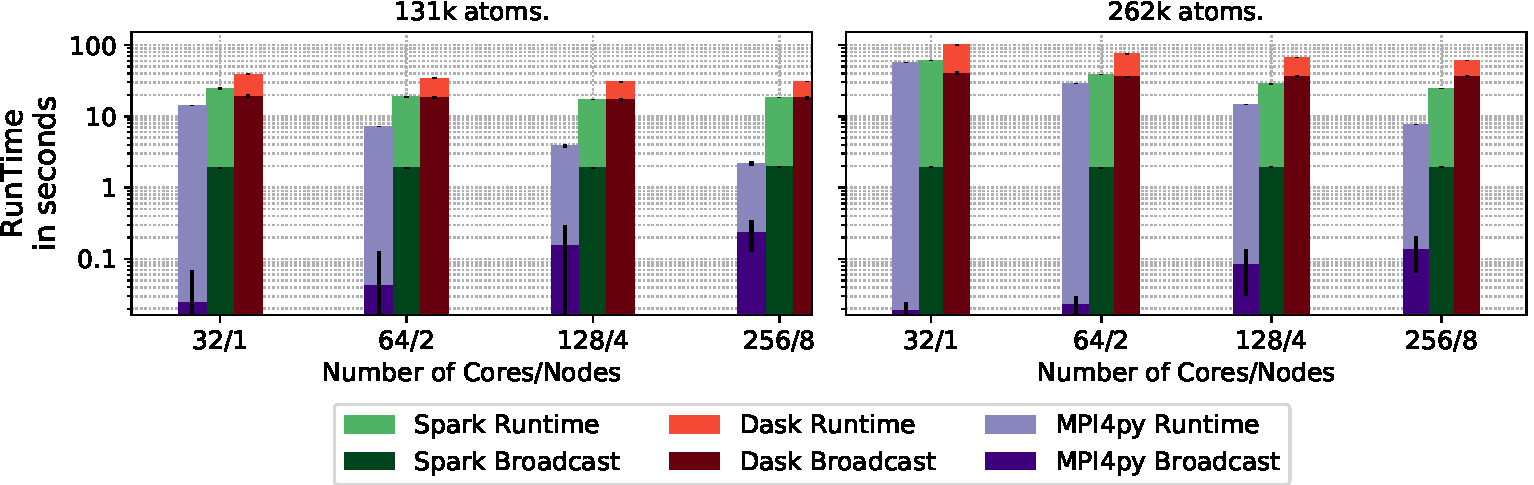
\includegraphics[width=.95\textwidth]{figures/data_analytics_hpc/task_par/spark_dask_lf_approach1.pdf}
    \caption{Broadcast and 1-D Partitioned Leaflet Finder (Approach 1).
    Runtime for multiple system sizes on different number of cores for Spark, Dask and MPI4py.}
    \label{fig:WranglerLeafLetFinderApp1}
\end{figure}

\subsubsection*{Broadcast and 1-D Partitioning}
Approach 1 utilizes a broadcast to distribute the data to all nodes, which is supported by Spark, Dask and MPI.
All nodes maintain a complete copy of the dataset.
Each \texttt{map} task computes the pairwise distance on its partition.
We use 1-D partitioning.
Figure~\ref{fig:WranglerLeafLetFinderApp1} shows the detailed results: as expected the usage of a broadcast has severe limitations for Spark and Dask.
MPI broadcast is a fraction of the overall execution time and significantly smaller than Spark and Dask.
MPI's broadcast times increase linearly as the number of processes increases, while Spark's and Dask's remain relatively constant for each dataset, due to more elaborate broadcast algorithms compared to MPI.
Broadcast times are about $3\%$ -- $15\%$ of the edge discovery time for Spark, $40\%$ -- $65\%$ for Dask, and $<1\%$ -- $10\%$ for MPI4py.
Spark offers a more efficient communication subsystem compared to Dask.
In addition, Dask broadcast partitions the dataset to a list where each element represents a value from the initial dataset.
This did not allow broadcasting the $524k$ atom dataset.
Nevertheless, the limited scalability of this approach due to transmitting the entire dataset renders it only usable for small datasets.
It shows the worst performance and scaling of all approaches for Spark, Dask and MPI4py.

Furthermore, this approach only scales up to $262k$ atoms for Dask, and $524k$ atoms for Spark and MPI4py on Wrangler.
Spark's performance is comparable to MPI4py for the $262k$, and $524k$ datasets.
It also shows better performance for the smallest core count in the $524k$ case.
Dask is at least two times slower than our MPI implementation.

%%%%%%%%%%%%%%% APPROACH 2 %%%%%%%%%%%%%%%%%%


\begin{figure}[t]
    \centering
    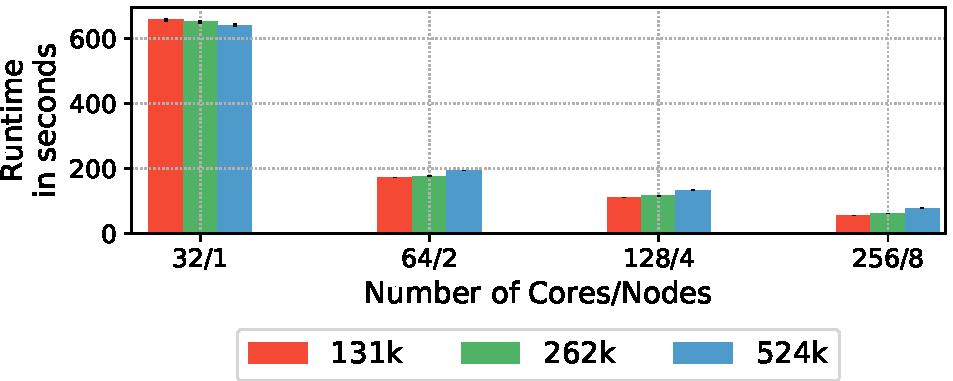
\includegraphics[width=.95\textwidth]{figures/data_analytics_hpc/task_par/rpLF.pdf}
    \caption{RADICAL~-Pilot Task API and 2-D Partitioned Leaflet Finder (Approach 2).
    Runtime for multiple system sizes over different number of cores.}
    %Overheads dominate since execution times are similar despite the system size.}
    \label{fig:rpLF}
\end{figure}

\subsubsection*{Task-API and 2-D Partitioning}
Approach~\ref{en:2} tries to overcome the limitations of approach 1, especially broadcasting and 1-D partitioning.
A 2-D block partitioning is essential, as it evenly distributes the compute and more efficiently utilizes the available memory.
2-D partitioning is not well supported by Spark and Dask.
Spark's RDDs are optimized for data-parallel applications with 1-D partitioning.
While Dask's array supports 2-D block partitioning, it was not used for this implementation.
We return the adjacency list of the graph instead of an array to fully use the capabilities of the abstraction.
Thus, each task works on a 2-D pre-partitioned part of the input data.

Figure~\ref{fig:All4approachesNoRp} shows the runtimes of approach~\ref{en:2} for Spark, Dask, MPI4py and Figure~\ref{fig:rpLF} for RADICAL~-Pilot.
As expected this approach overcomes the limitations of approach 1 and can easily scale to larger datasets (e.\,g., $524k$ atoms) while improving the overall runtime.
Dask's execution time was smaller by at least a factor of two.
However, we were not able to scale this implementation to the 4M dataset, due to memory requirements of \texttt{cdist}.
For RADICAL~-Pilot we observed significant task management overheads (see also section~\ref{sec:framework_eval}).
This is a limitation of RADICAL~-Pilot with respect to managing large numbers of tasks.
This is particularly visible when the scenario was run on a single node with 32 cores.
As more resources become available, i.e. more than 64 cores, the performance improves dramatically.

Furthermore, Spark and Dask did not scale as well as MPI, which achieved linear speedups of $\sim8$ when using $256$ cores.
Spark and Dask achieved maximum speedups of $4.5$ and $\sim5$ respectively.
Despite this fact, both frameworks had similar performance on $32$ cores for the $262k$ and $524k$ datasets.

%%%%%%%%%%%%%% Approach 3 %%%%%%%%%%%%%%%%%%%%%%%

\subsubsection*{Parallel Connected Components}
Communication between the edge discovery and connected components stages is another important aspect.
The edge discovery phase output for the $524k$ atoms dataset is $\approx$ $100\,\textup{MB}$.
To reduce the amount of data that need to be shuffled, we refined the algorithm to compute the graph components on the partial dataset in the \texttt{map} phase.
The partial components are then merged in a \texttt{reduce} phase.
This reduces the amount of shuffle data by more than $50\%$ (e.\,g., to $12\textup{MB}$ for Spark and $48\textup{MB}$ for Dask).
Figure~\ref{fig:All4approachesNoRp} shows the improvements in runtime, by $\sim20\%$ for Spark and Dask, but not MPI4py.
Further, we were able to run very large datasets, such as the 4M dataset, using this architectural approach using Spark and MPI4py.
Dask was restarting its worker processes because their memory utilization was reaching $95\%$.

Spark, and Dask have comparable performance with MPI on 32 cores, which utilizes a single node on Wrangler.
However, the MPI4py implementation scales almost linearly for all datasets, Spark and Dask cannot, reaching a maximum of $\sim5$ for the three smaller datasets.
In addition, Spark is able to scale almost linearly for the $4M$ atoms dataset providing comparable performance to MPI4py.

%%%%%%%%%%%%%% Approach 4 %%%%%%%%%%%%%%%%%%%%%%%

\subsubsection*{Tree-Search}
A bottleneck of approaches~\ref{en:1},~\ref{en:2} and~\ref{en:3} is the edge 
discovery via the naive calculation of the distances between all pairs of atoms. 
In approach~\ref{en:4}, we replace the pairwise distance function with a tree-based, 
nearest neighbor search algorithm, in particular BallTree~\cite{omohundro89five}. 
The algorithm: 
\begin{inparaenum}
    \item constructs of a tree, and
    \item queries for neighboring atoms.
\end{inparaenum}

Using tree-search, the computational complexity can be reduced from $n^2$ to $log$. 
We use a BallTree as offered by Scikit-Learn~\cite{scikit-nearest} for our implementation.

Figure \ref{fig:All4approachesNoRp} illustrates the performance of the implementation.
For small datasets, i.\,e., $131k$ and $262k$ atoms, approach~\ref{en:3} is faster than the tree-based approach, since the number of points is too small.
For the large datasets, the tree approach is faster.
In addition, the tree has a smaller memory footprint than \texttt{cdist}.
This allowed to scale to larger problems, e.\,g., a $4M$ atoms and $44.6M$ edges dataset without changing the total number of tasks.

Dask shows better scaling than Spark for $131k$, $262k$, and $524k$ atoms.
This is not true for $4M$ atoms, indicating that Dask's communication layer is not able to scale as well as Spark's.
Spark shows similar performance with MPI4py for the largest dataset due to minimal shuffle traffic.
Thus, MPI's efficient communication does not become relevant.

\section{Task-Parallel Framework Selection Conceptual Model and Discussion}
In this section we provide a conceptual model that allows application developers to carefully select a framework according to their requirements (e.\,g., compute and I/O).
It is important to understand both the properties of the application and Big Data frameworks.
Table~\ref{tab:framework} illustrates the criteria of this conceptual model and ranks the three frameworks.

\begin{table}[t]
    \centering
    \begin{tabular}{@{}cccc@{}}
        \toprule
        &\textbf{RADICAL~-Pilot}     &\textbf{Spark} &\textbf{Dask}\\
        \multicolumn{4}{l}{\textbf{Task Management}} \\
        \midrule
        Low Latency   &- &o &+\\
        Throughput    &- &+ &++\\
        MPI/HPC Tasks &+ &o &o\\
        Task API   &+ &o &++\\
        Large Number of Tasks   &-- &++ &++\\\hline
        \multicolumn{4}{l}{\textbf{Application Characteristics}}\\\midrule
        Python/native Code &++ &o &+\\
        Java               &o &++ &o\\
        Higher-Level Abstraction &- &++ &+\\
        Shuffle                  &- &++ &+\\
        Broadcast                &- &++ &+\\
        Caching                  &- &++ &o\\
        \bottomrule
    \end{tabular}
    \caption{Task-parallel framework selection decision methodology: Criteria and Ranking for Framework Selection. -~: Unsupported or low performance
        +~: Supported, ++~: Major Support, and o~:Minor support.\label{tab:framework}}
\end{table}
%  application perspective

\subsubsection*{Application Perspective}
We showed that we can implement MD trajectory data analysis applications using all three frameworks, as well as MPI4py.
Implementation aspects, such as computational complexity, and shuffled data size influence the performance greatly.
For embarrassingly parallel applications with coarse grained tasks, such as PSA, the choice of the framework does not significantly influence performance (Figures~\ref{fig:HausdorffWrangler} and~\ref{fig:comet_wrangler_haus}).
In addition, the performance difference against MPI4py was not significant (Figures~\ref{fig:HausdorffWrangler} and~\ref{fig:comet_wrangler_haus}).
Thus, aspects, such as programmability and integrate-ability, become more important.

For fine-grained data parallelism, a Big Data framework, such as Spark and Dask, clearly outperforms RADICAL~-Pilot (Figures~\ref{fig:All4approachesNoRp},~\ref{fig:rpLF}).
If coupling is introduced, i.\,e. task communication is required (e.\,g., reduce), using Spark becomes advantageous (Approaches~\ref{en:3} \& \ref{en:4}). 
PI4py outperformed Dask, and Spark, despite both frameworks scaling for the larger datasets.
Especially Spark was able to provide linear speedup for approach~\ref{en:3} of Leaflet Finder (Figure~\ref{fig:All4approachesNoRp}).
Integrating with frameworks that provide higher level abstractions provides scalable solutions for more complex algorithms.
However, integrating Spark with other tools needs to be carefully considered.
The integration of Python tools, e.\,g. MDAnalysis, often causes overheads due to the frequent need for serialization and copying data between the Python and Java space.

Dask had the smallest learning curve of all three frameworks.
As a result, it allows for faster prototyping compared to RADICAL~-Pilot and Spark.
RADICAL~-Pilot's learning curve is more steep, but is more versatile than Dask and Spark, by offering the lowest level abstraction. 
Spark had the slowest learning curve.
It required tuning to get the number of tasks correctly, as well as argument passing to map and reduce functions.

\subsubsection*{Framework Perspective}
RADICAL~-Pilot is well suited for HPC applications, e.\,g., ensembles (up to $50k$ tasks) of parallel MPI applications, as shown in Ref.~\cite{merzky2018design,merzky2019using}.
It has limited scalability when supporting large numbers of short-running tasks, as often found in data-intensive workloads.
The file staging implementation of RADICAL~-Pilot is not suitable for supporting the data exchange patterns, i.e. shuffling, required for these applications.
However, executing MPI and Spark applications alongside on the same resource makes RADICAL~-Pilot particularly suitable when different programming models need to be combined.

% framework perspective
Dask provides a highly flexible, low-latency task management and excellent support for parallelizing Python libraries.
We established that Dask has higher throughput (Figures~\ref{fig:dask_spark_rp_wrangler} and~\ref{fig:RP_Dask_Spark_throughput}).
However, Spark provides better speedups for the largest datasets compared to Dask (Figure ~\ref{fig:All4approachesNoRp}).
Dask's broadcast (Leaflet Finder approach~\ref{en:1}) and shuffle (Leaflet Finder approaches~\ref{en:2}-~\ref{en:4}) performance is worse for larger problems compared to Spark.
Thus, Dask's communication layer shows some weaknesses that are particularly visible during broadcast and shuffle.
Spark needs to be particularly considered for shuffle-intensive applications.
Its in-memory caching mechanism is particularly suited for iterative algorithms that maintain a static set of data in-memory and conduct multiple passes on that set.
